\section{Physical Model}

\begin{frame}
	\frametitle{Lagrange Formalism}
	\onslide<1->
	Method to describe dynamics of an accelerated system\\
	\begin{small}
	\begin{tabular}{ll}
		 & \\
		T & kinetic energy\\
		V & potentials\\
		F & non-conservative external forces\\
		r & points of actions of forces F\\ %position vector
		q & free variables\\
		Q & generalized forces\\ \\
	\end{tabular}
	\end{small}
	
	\onslide<2>
	\begin{align*}
	&\frac{d}{dt}\left(\frac{\partial T}{\partial \dot{q}_i}\right) -
	\frac{\partial T}{\partial q_i} +
	\frac{\partial V}{\partial q_i}
	= Q_i \\
	& Q = \left(\frac{\partial r}{\partial q}\right)^T F\\
	\end{align*}
		
\end{frame}	

\begin{frame}
	\frametitle{Physical Model of Excavator}
	
	%left, bottom, right, top
	%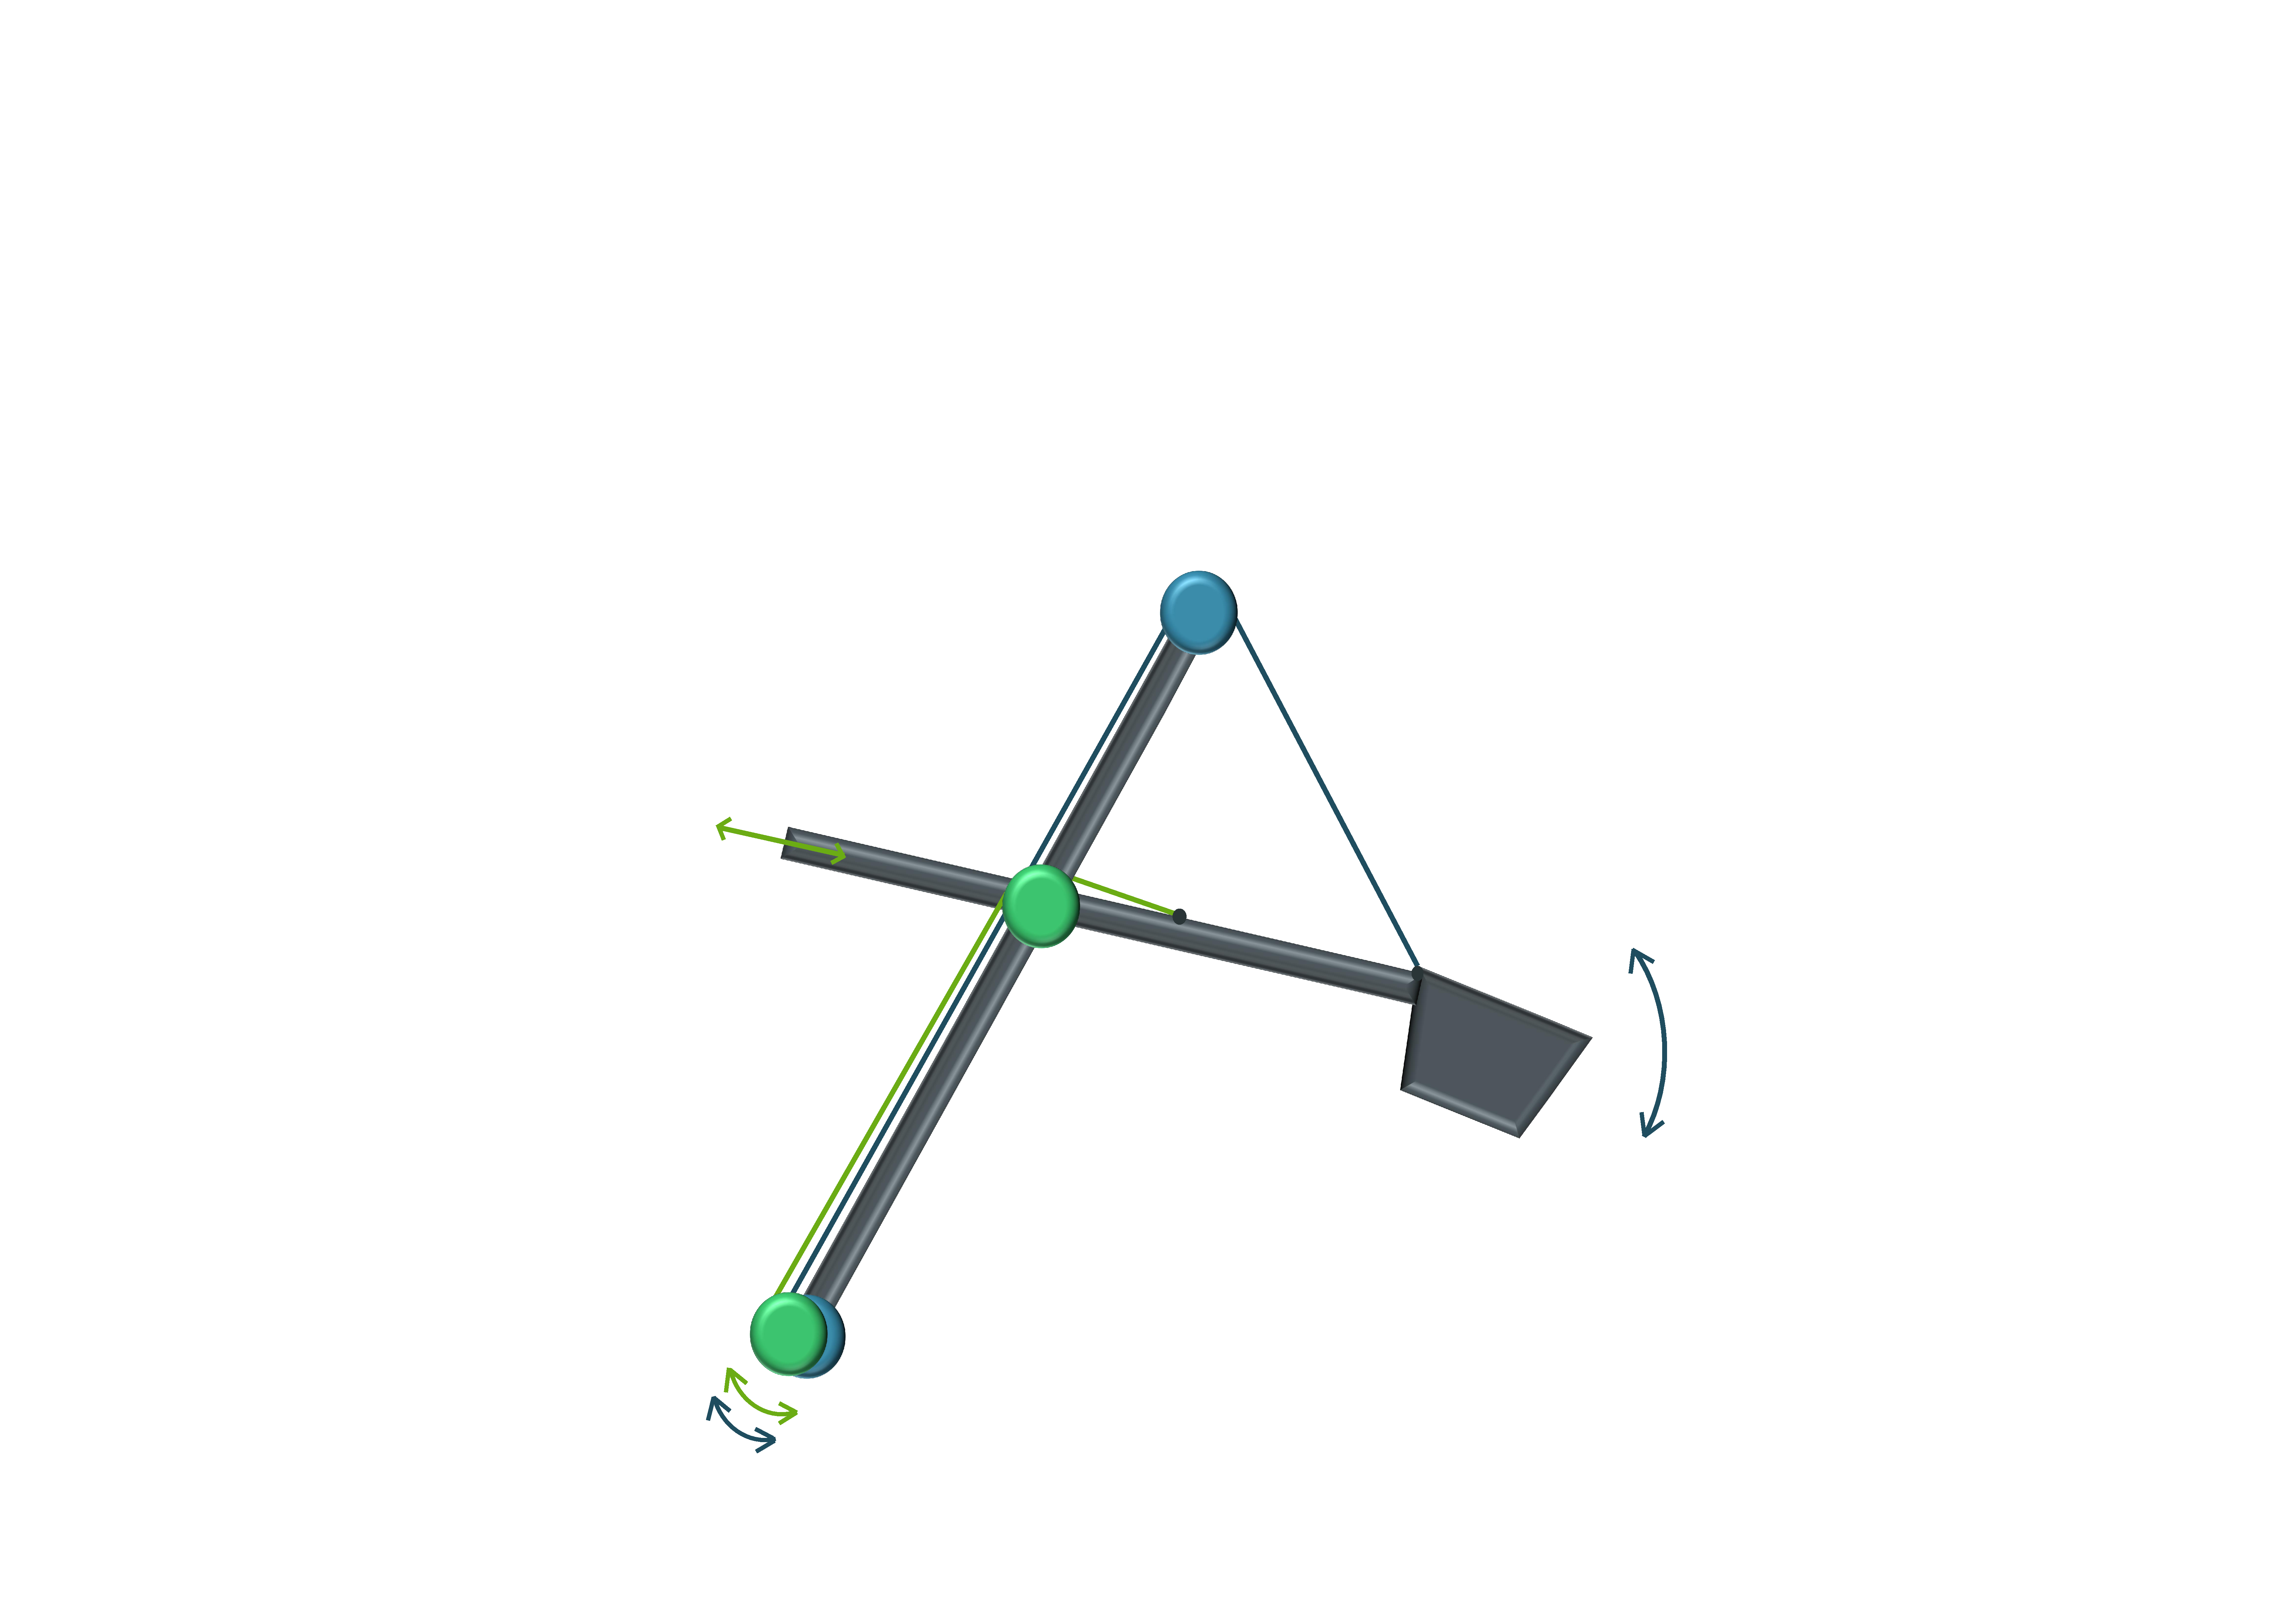
\includegraphics[trim=22cm 5cm 2cm 23cm, clip=true, width=\linewidth]{img/Excavator_Only}
	
	\begin{columns}
		\column{.6\linewidth}
			\centering
			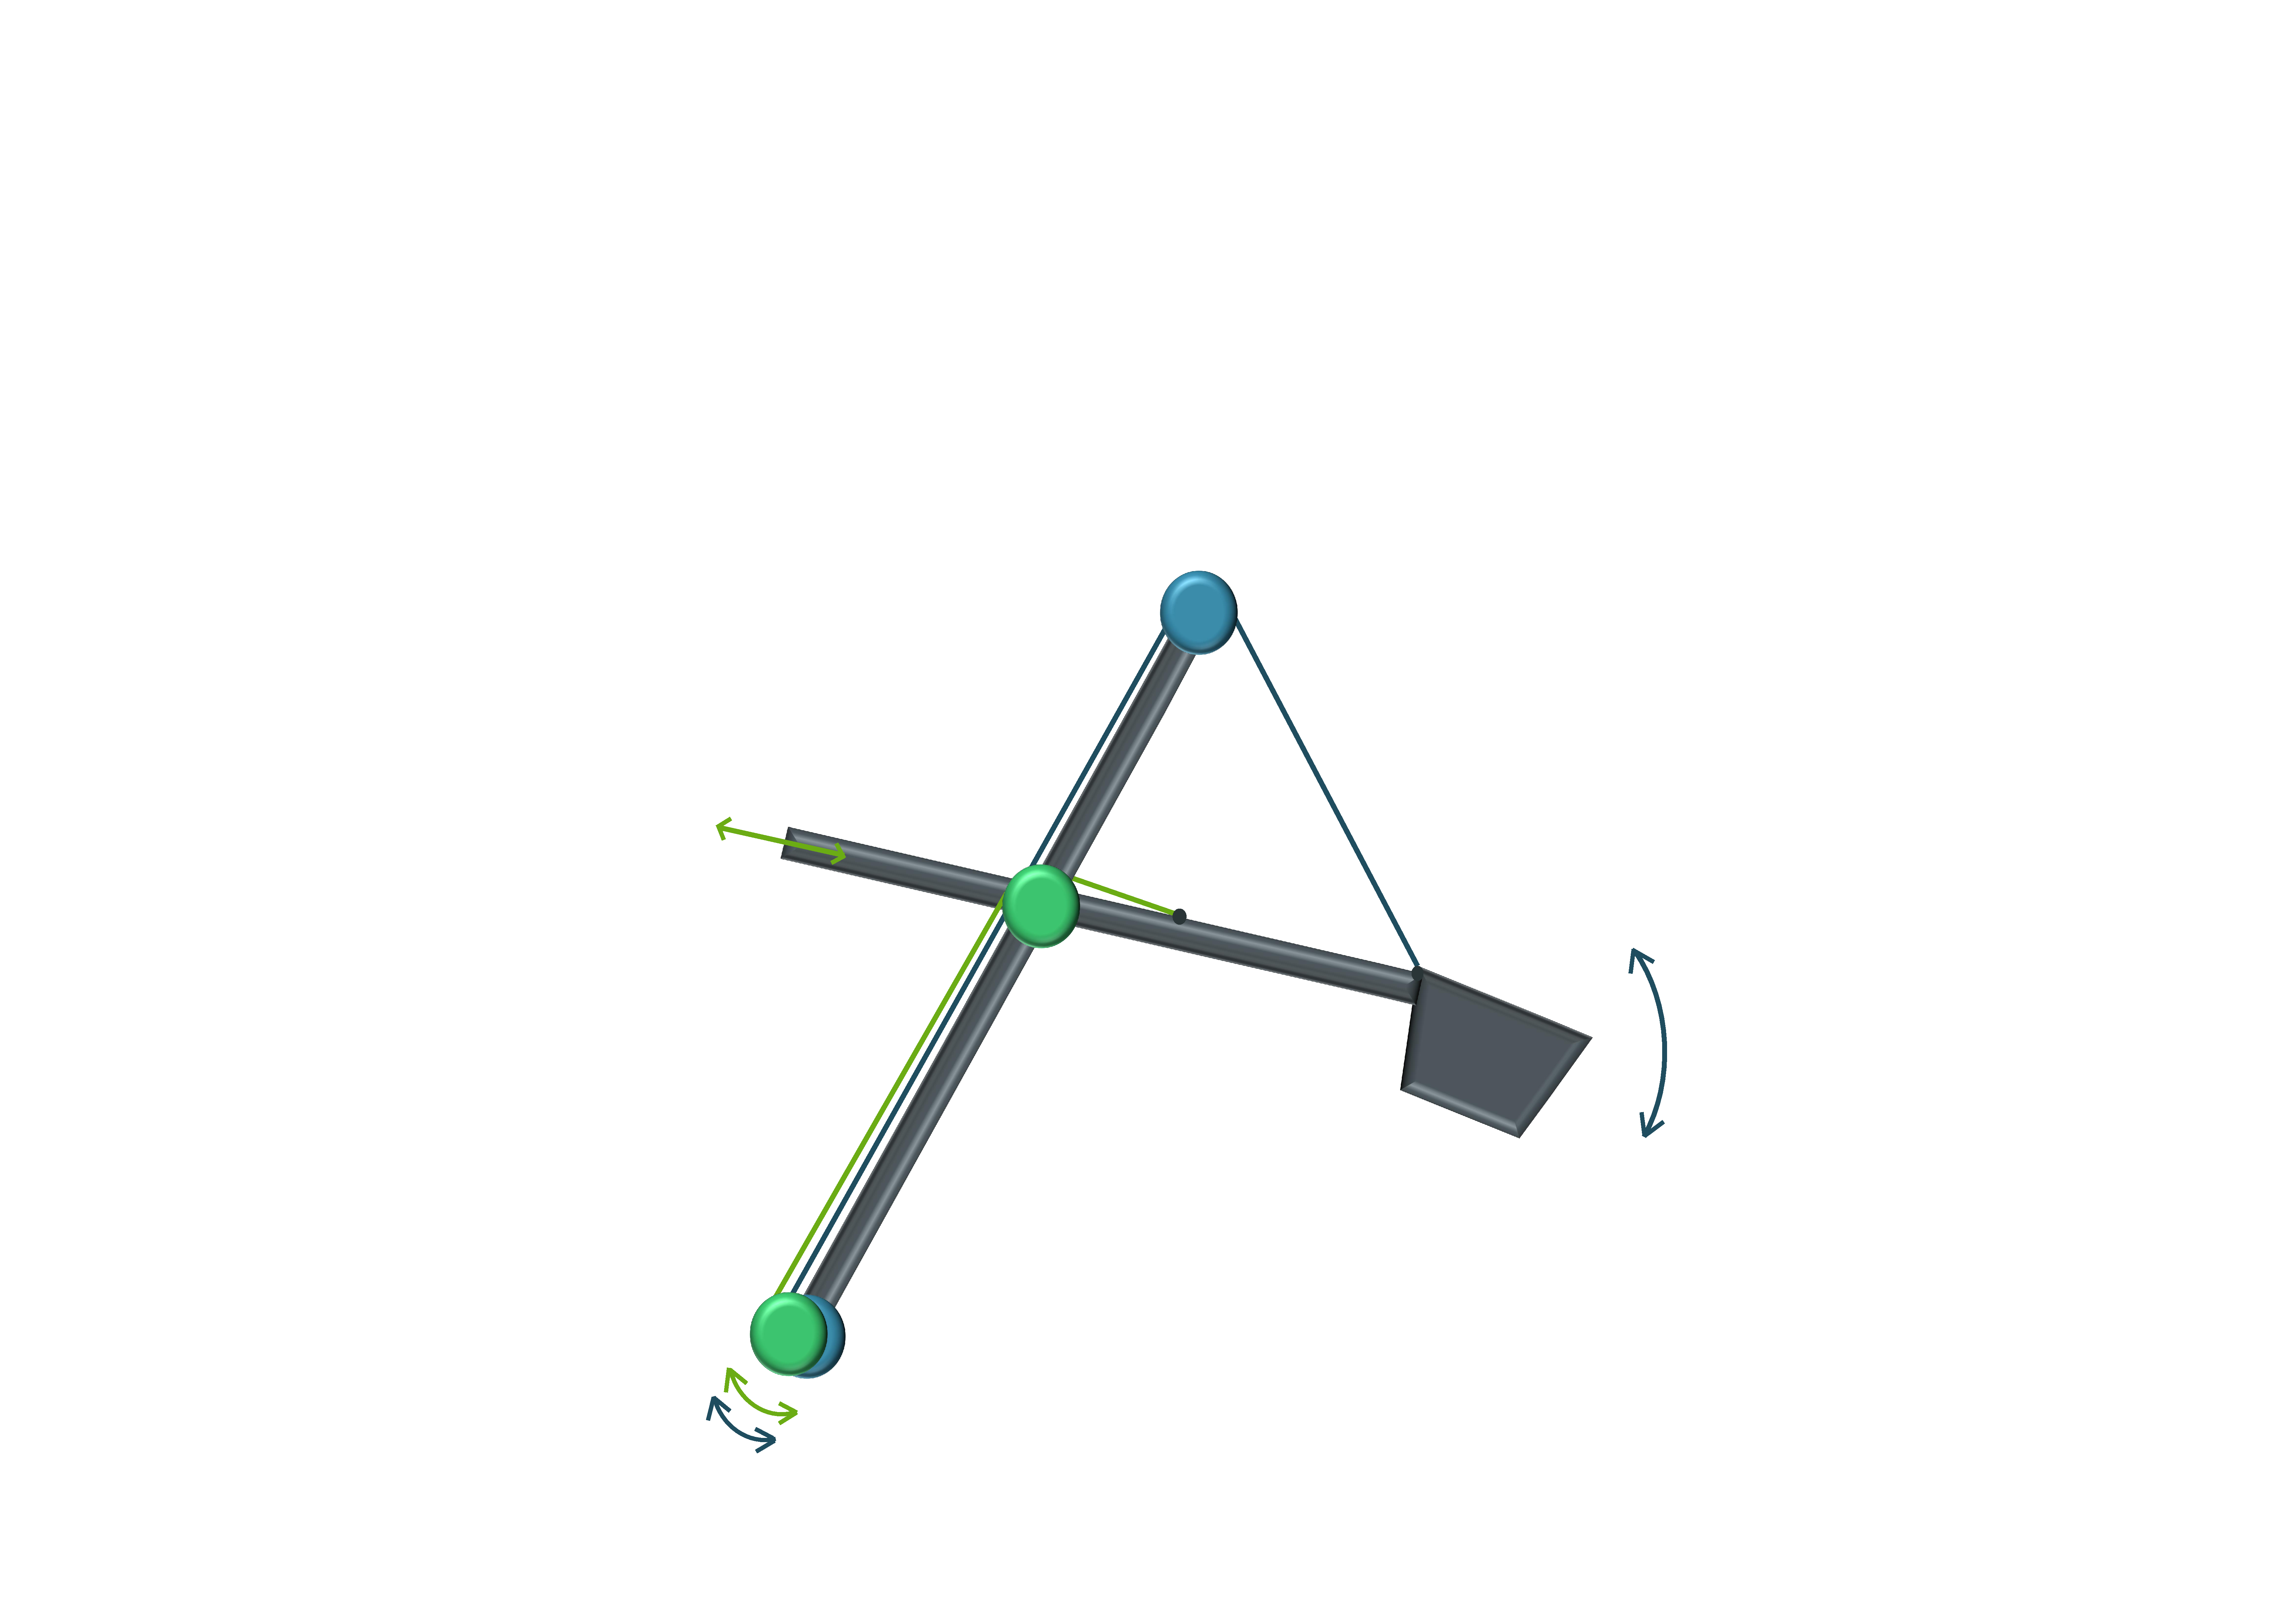
\includegraphics[trim=30cm 5cm 30cm 23cm, clip=true, width=\linewidth]{img/Excavator_Only}
		\column{.4\linewidth}
	\end{columns}
	
\end{frame}

\begin{frame}
	\frametitle{Physical Model of Excavator}
	
	%	invariant under transformation of coordinates $\rightarrow$ appropriate choice of 	coordinate system
	
	%first fix coordinate system $\rightarrow$ consider positions vectors, coordinates of mass points,... in this system\\
	
	%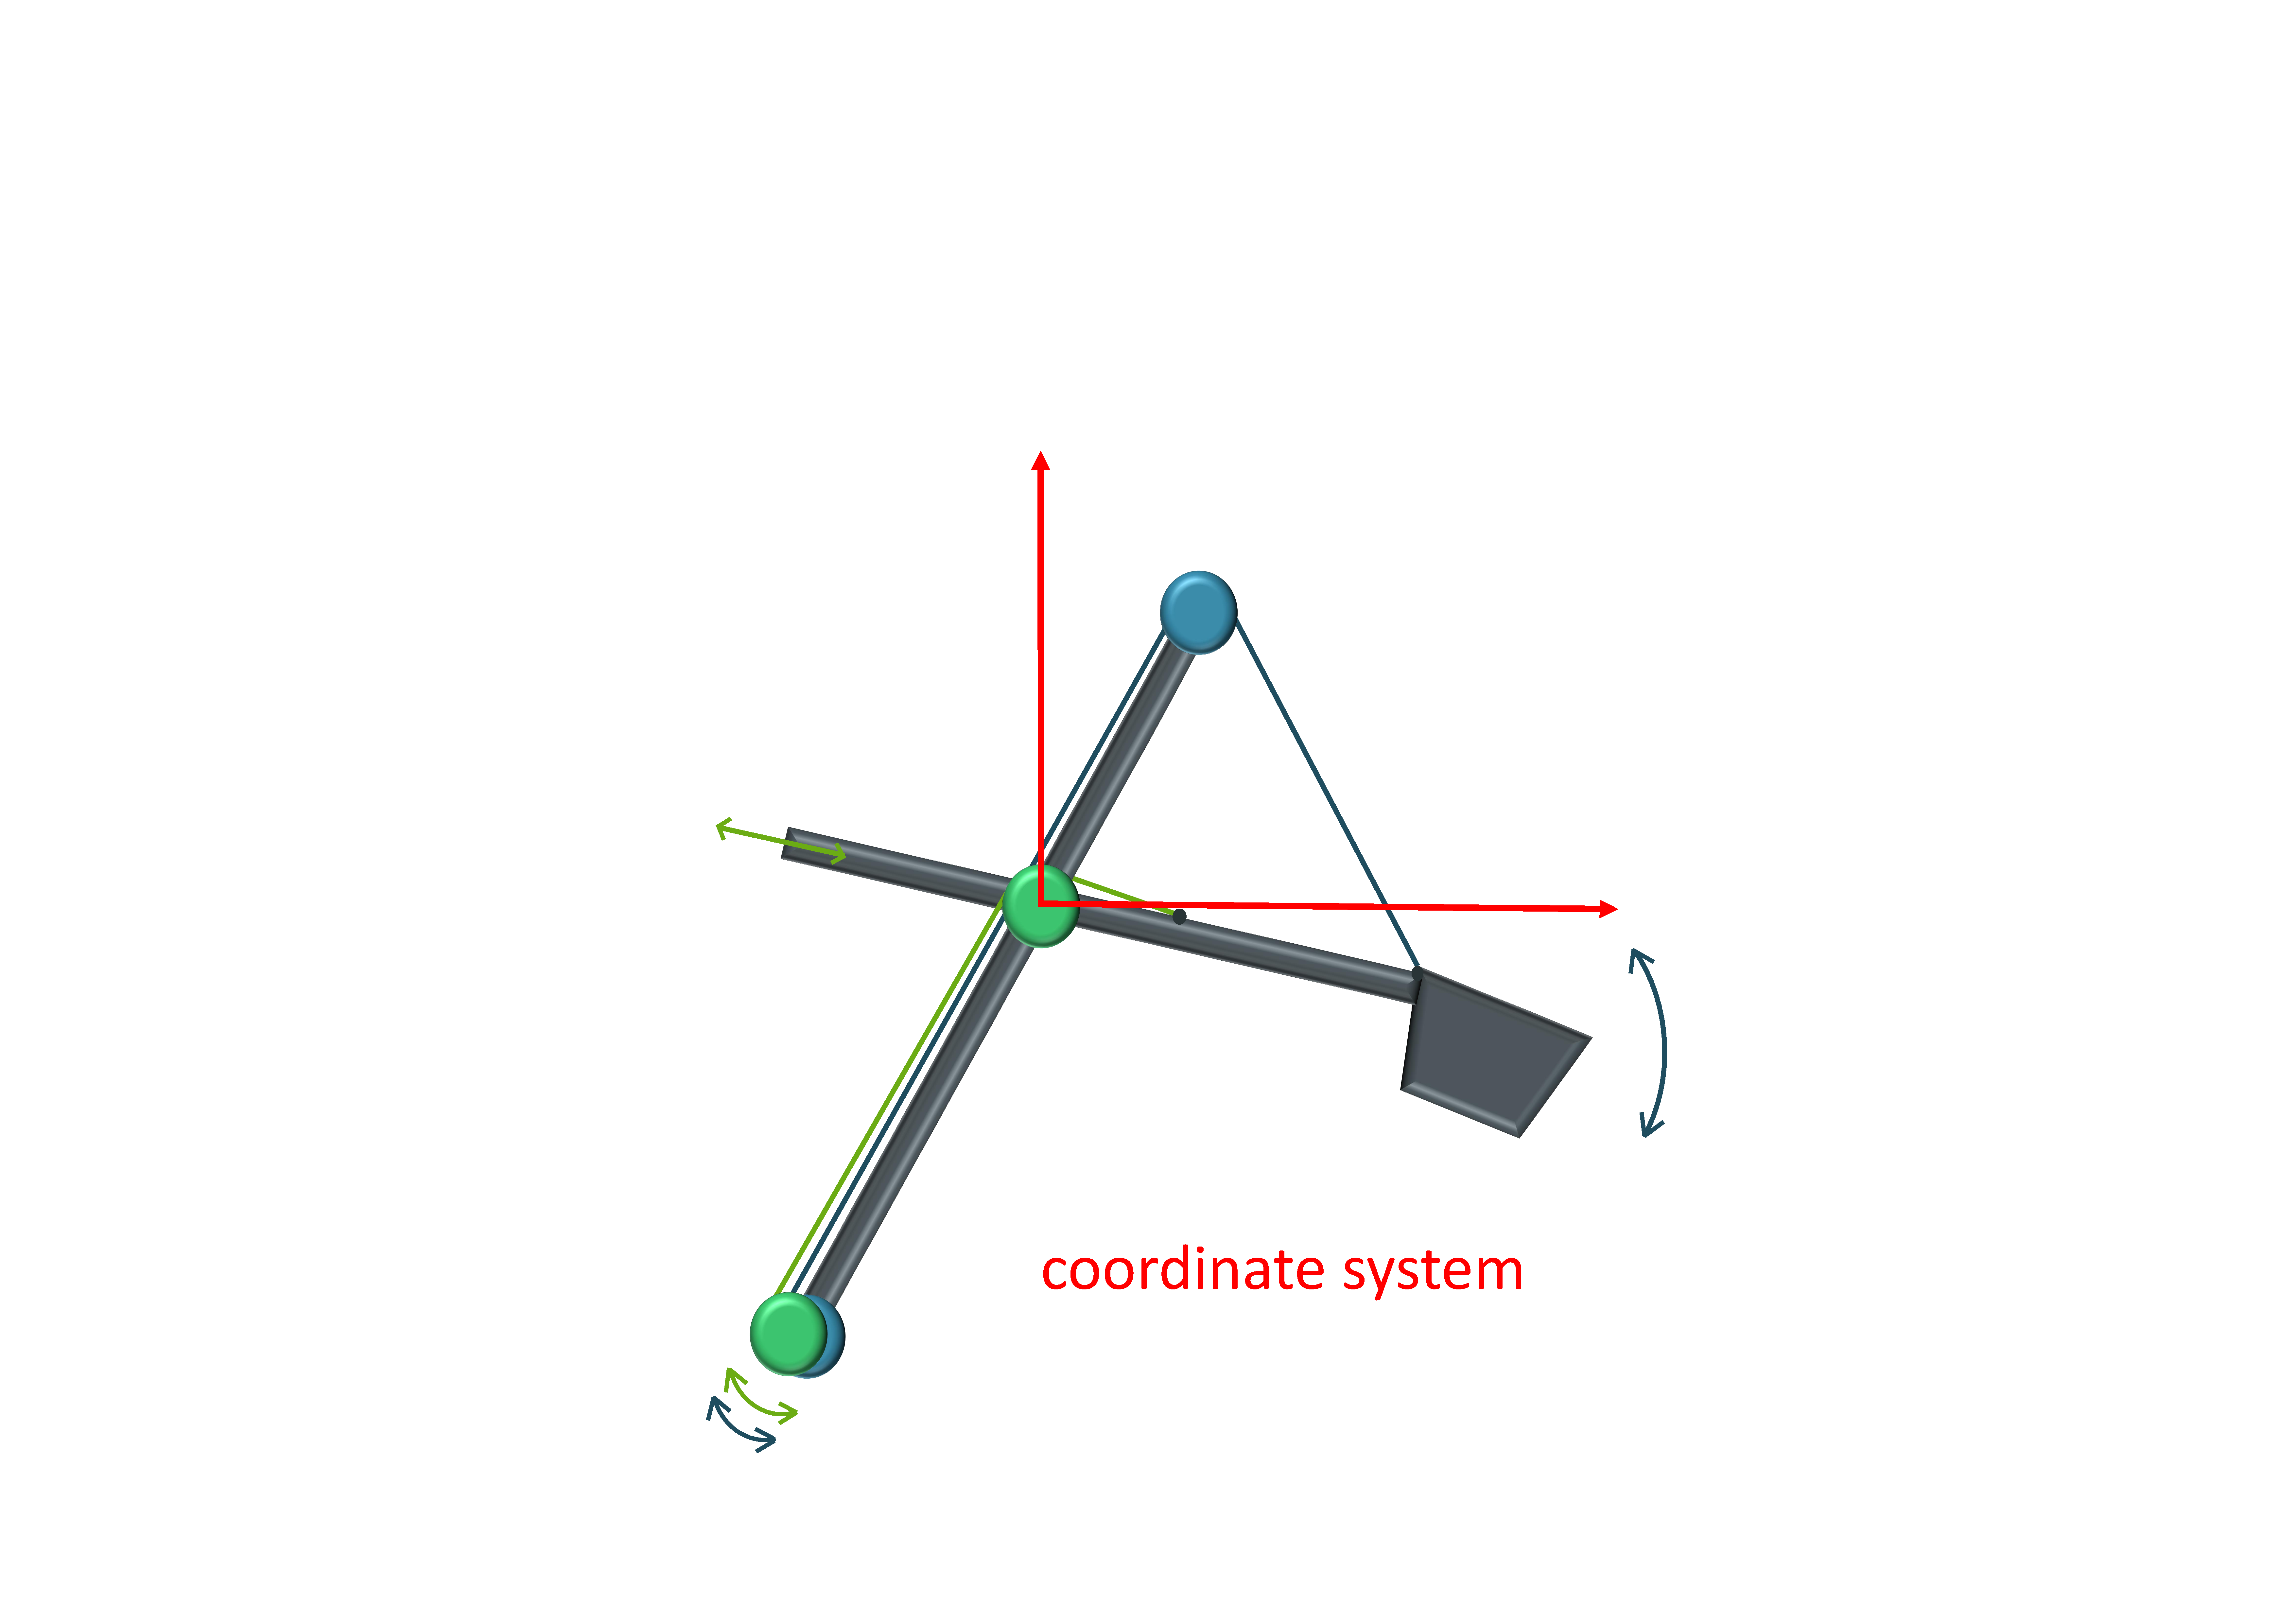
\includegraphics[trim=22cm 5cm 2cm 23cm, clip=true, width=\linewidth]{img/Excavator_coordinates2}
	
	\begin{columns}
		\column{.6\linewidth}
			\centering
			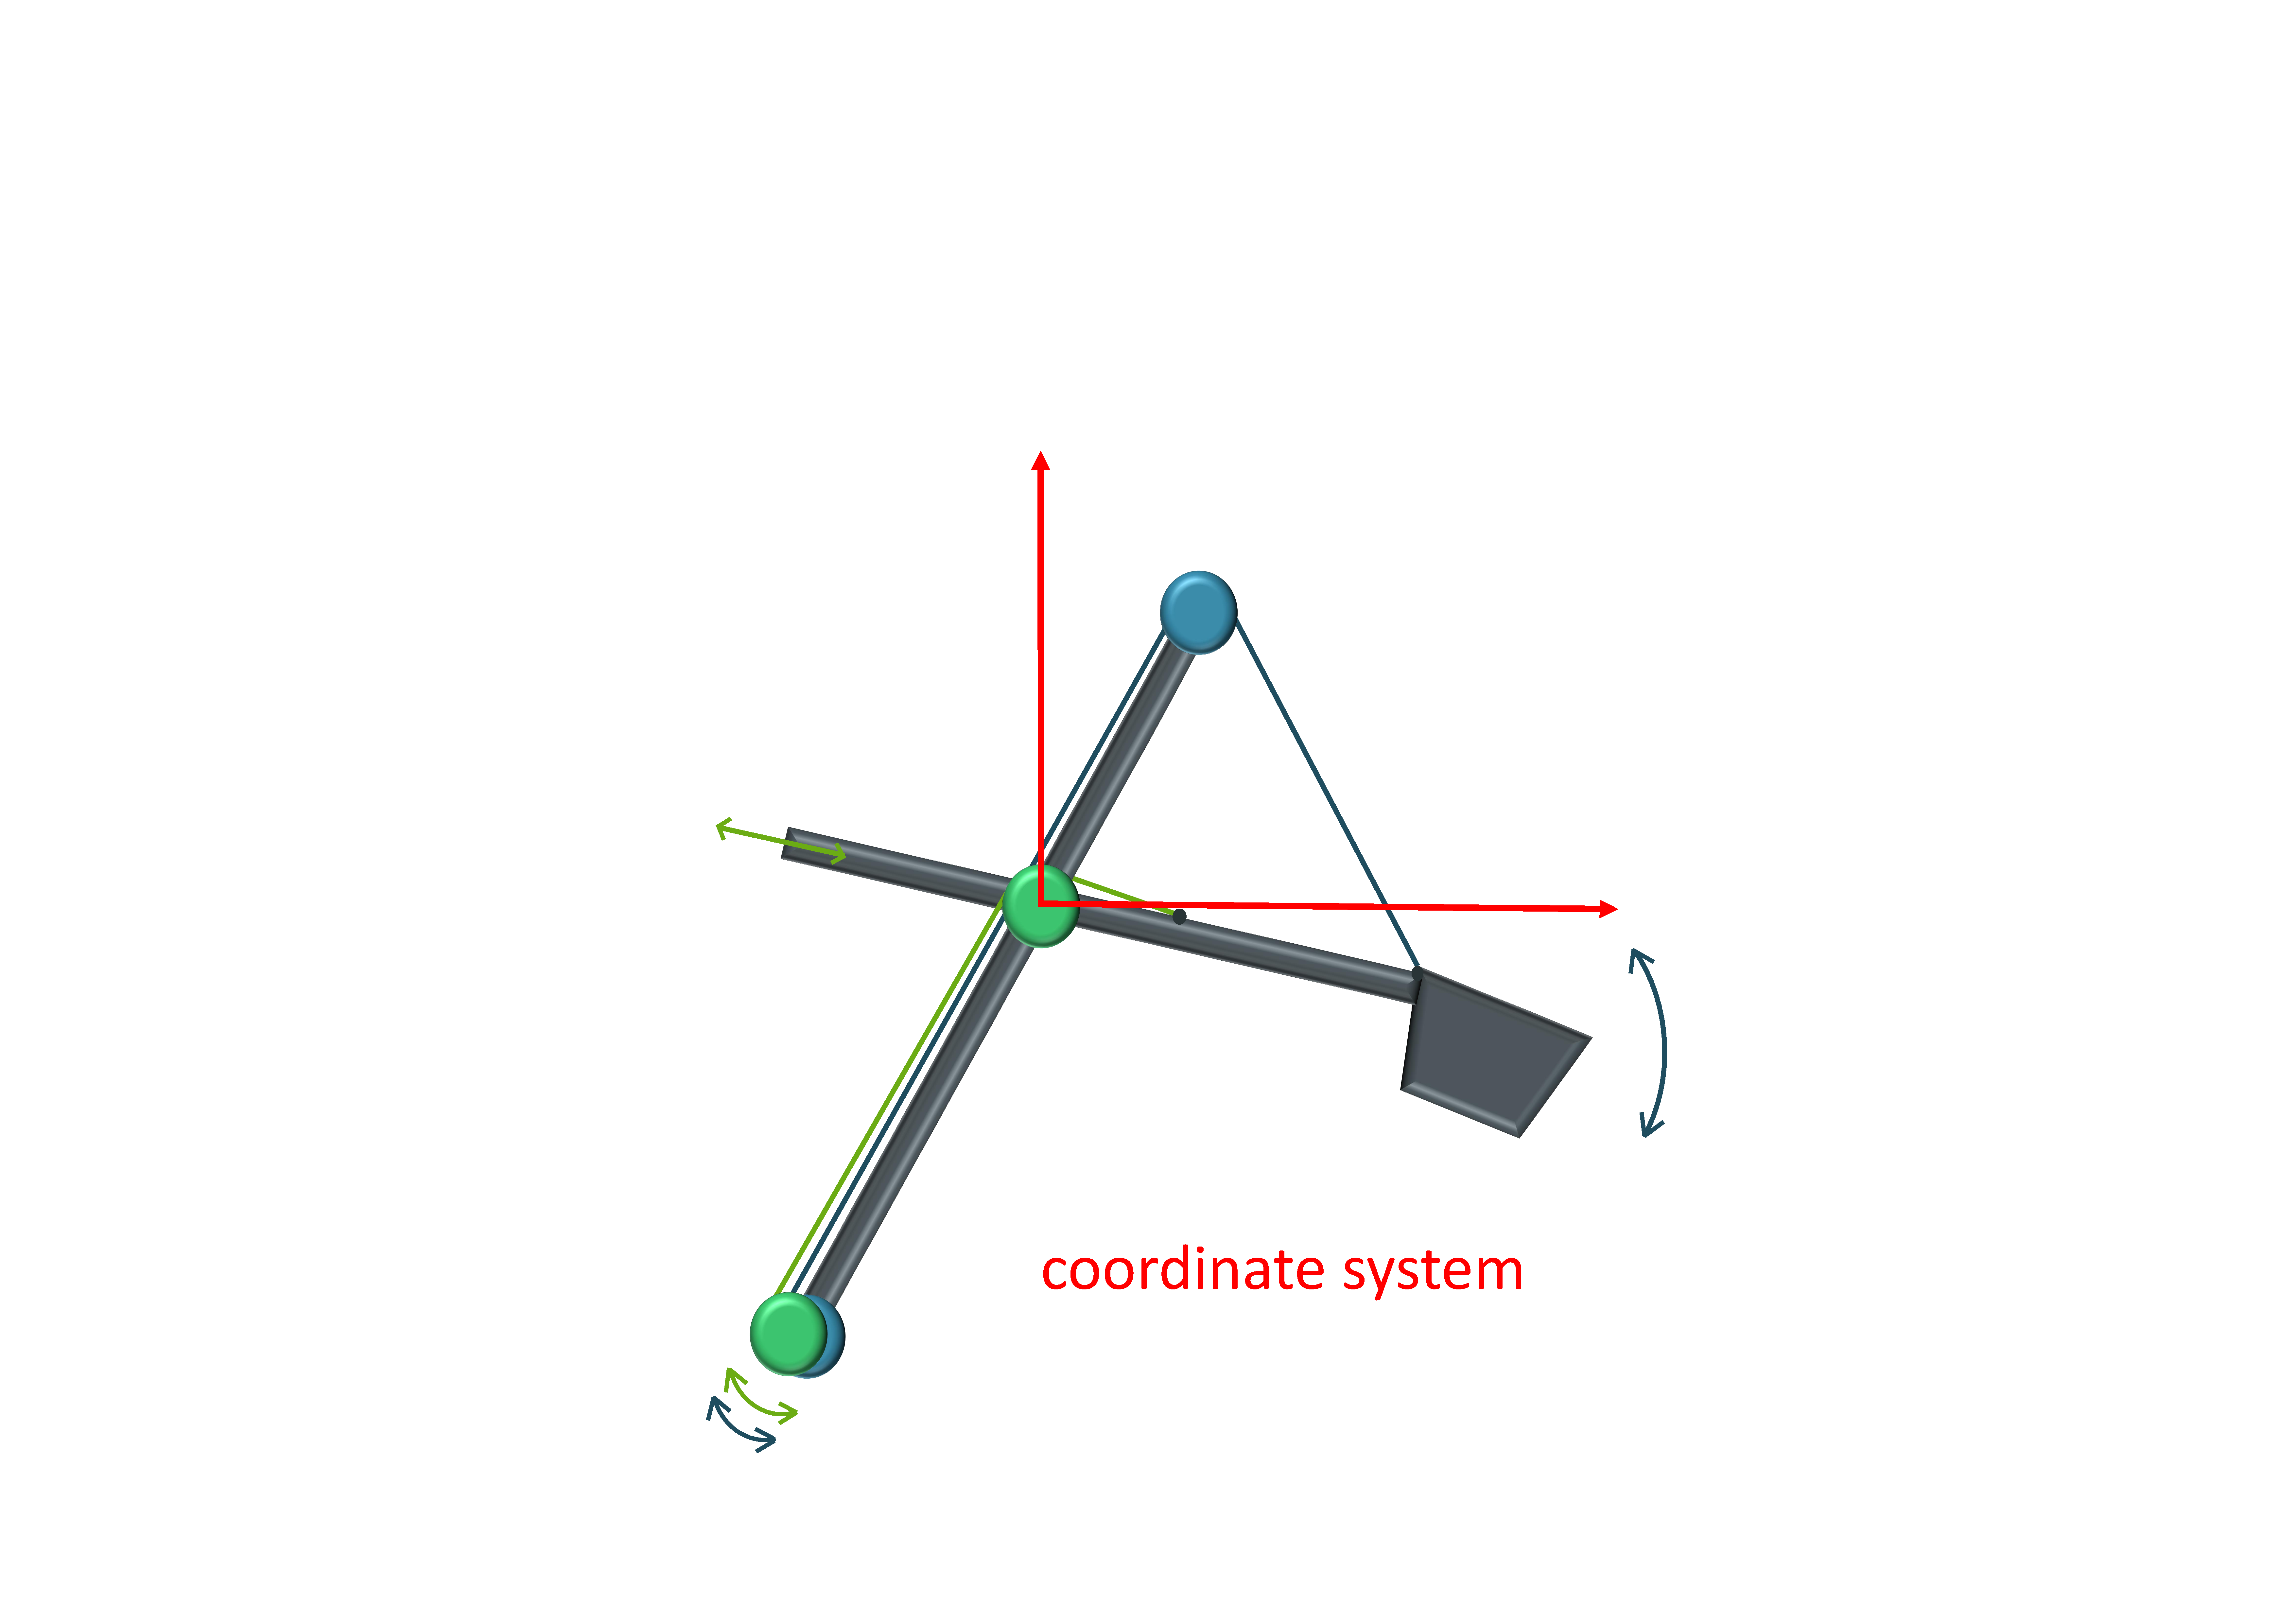
\includegraphics[trim=30cm 5cm 30cm 23cm, clip=true, width=\linewidth]{img/Excavator_coordinates2}
		\column{.4\linewidth}
			coordinate system
	\end{columns}
	
\end{frame}

\begin{frame}
	\frametitle{Physical Model of Excavator}
	
	%think of degrees of freedom $\rightarrow$ angle and length side arm $\rightarrow$ forces in the system will depend on excavator configuration and therefore on $s$ and $\theta$\\
	
	%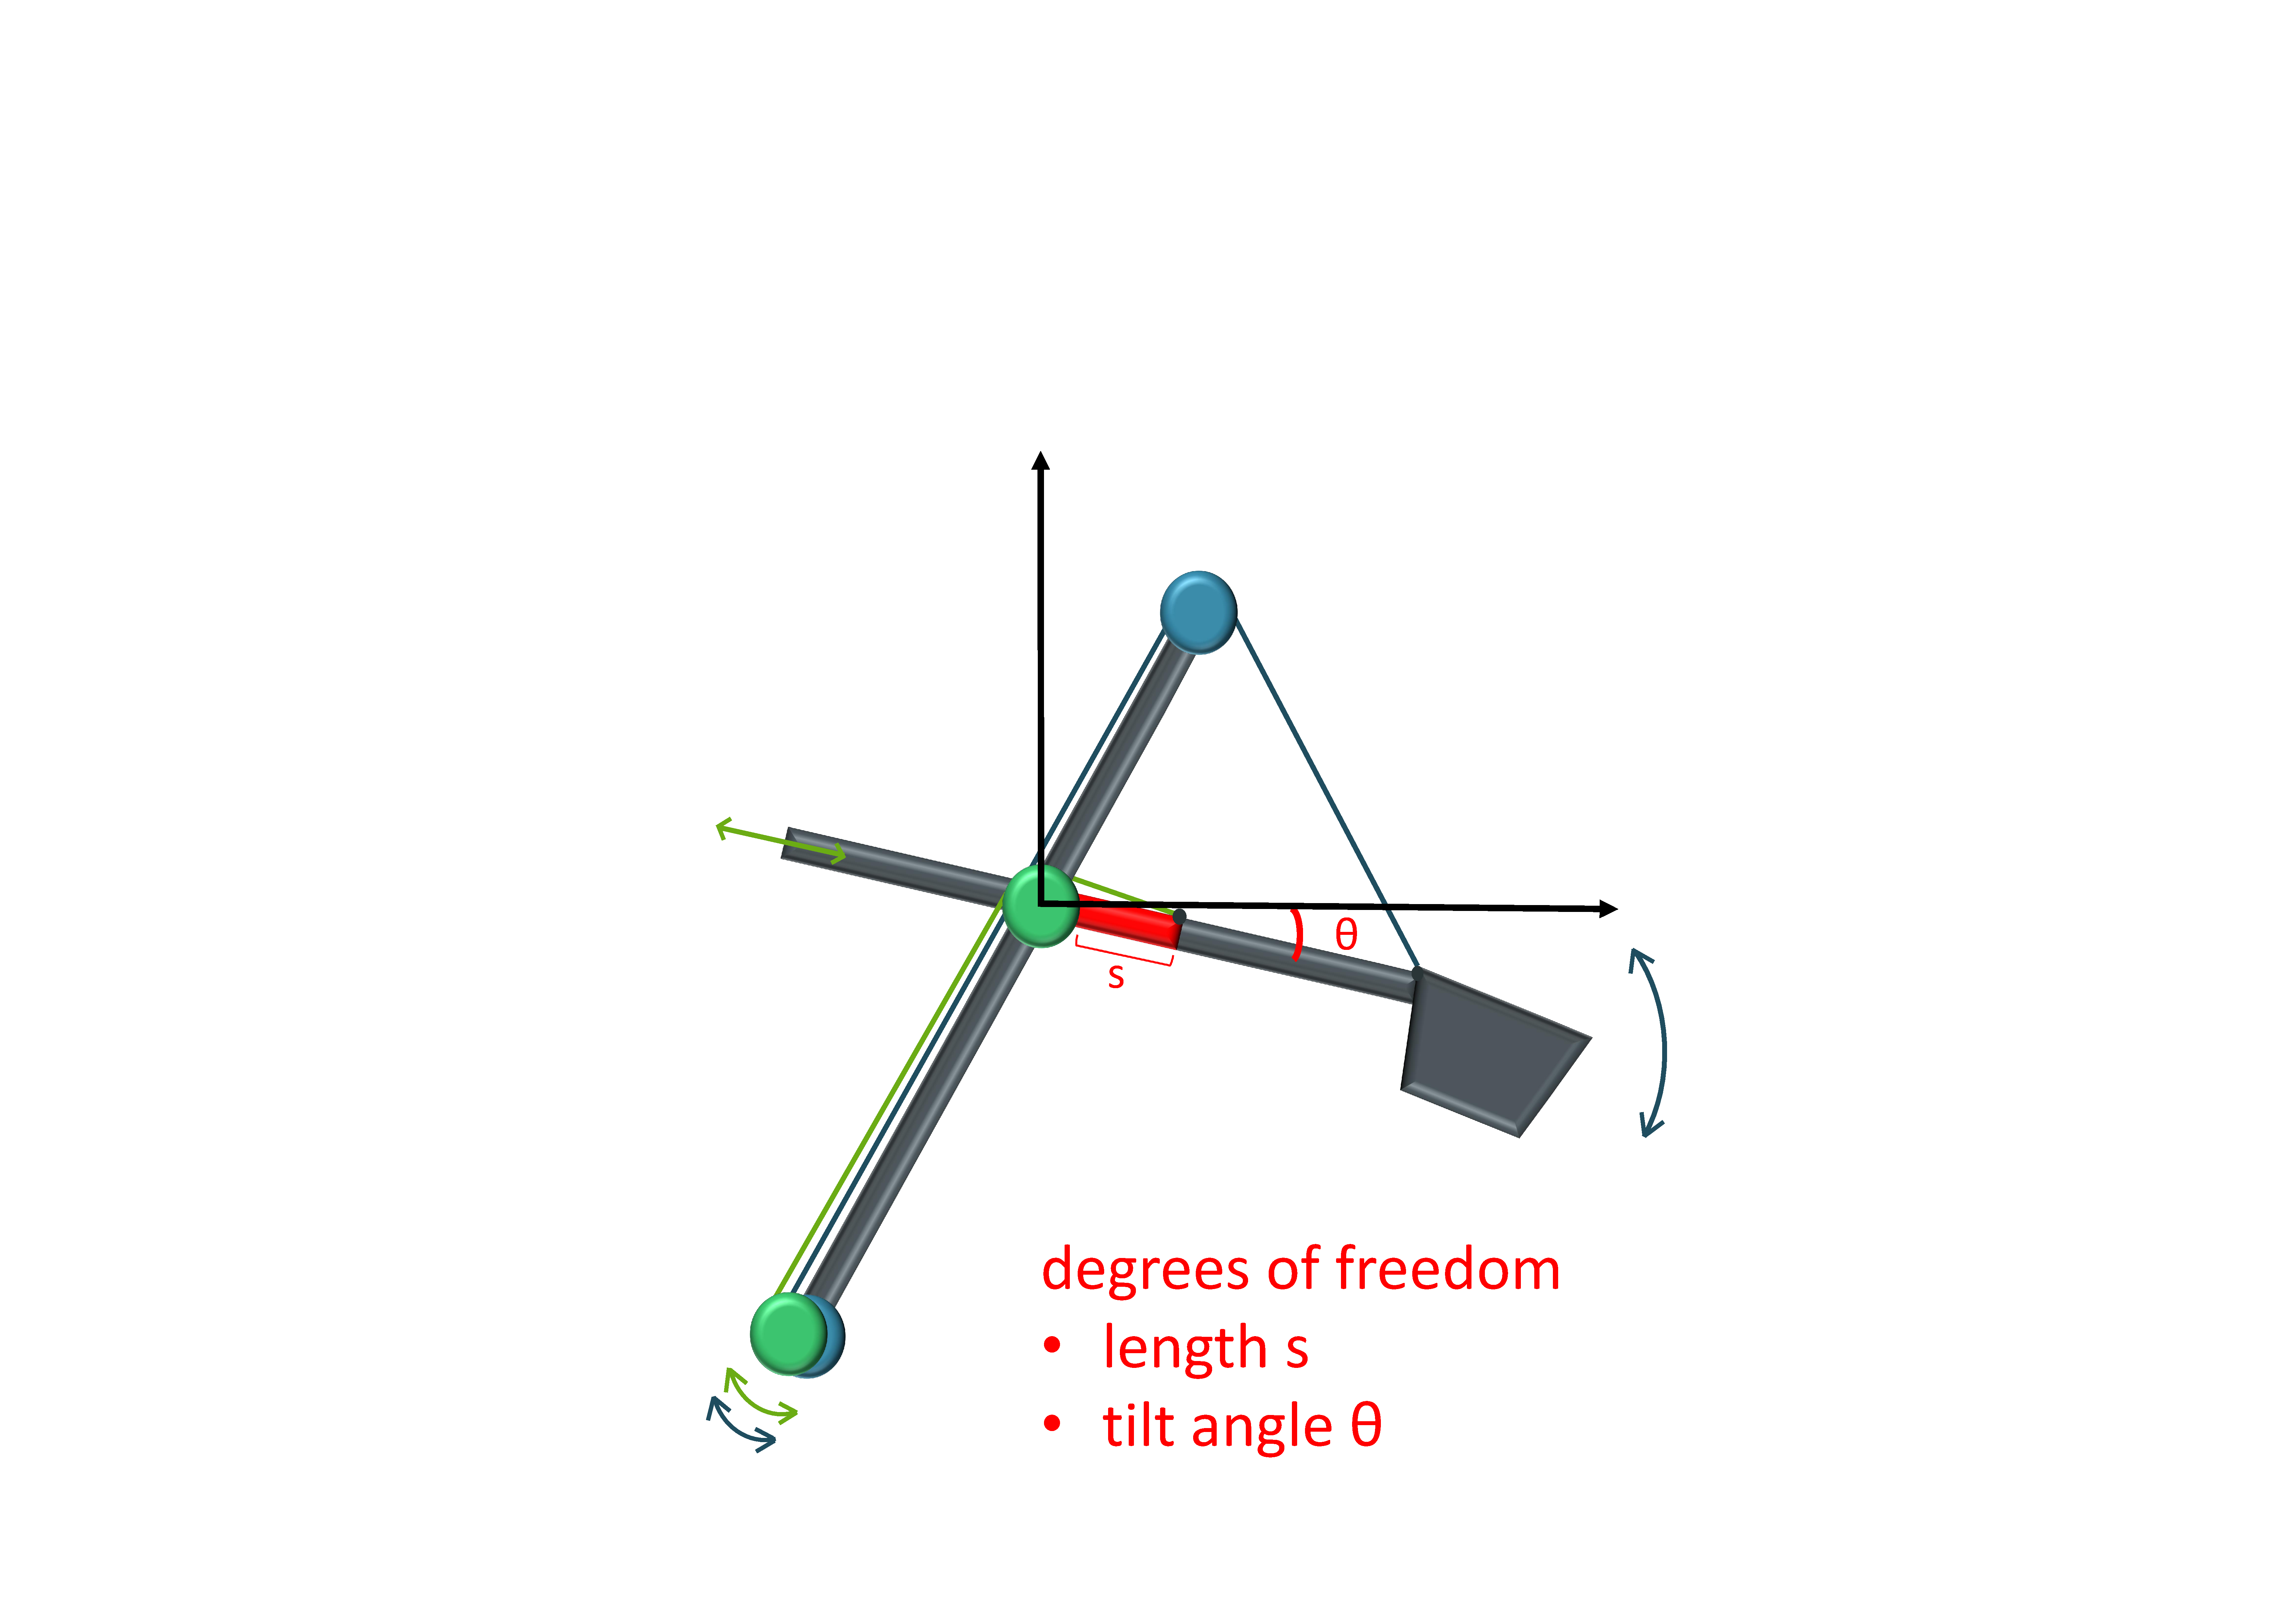
\includegraphics[trim=22cm 5cm 2cm 23cm, clip=true, width=\linewidth]{img/Excavator_dof2}
	
	\begin{columns}
		\column{.6\linewidth}
			\centering
			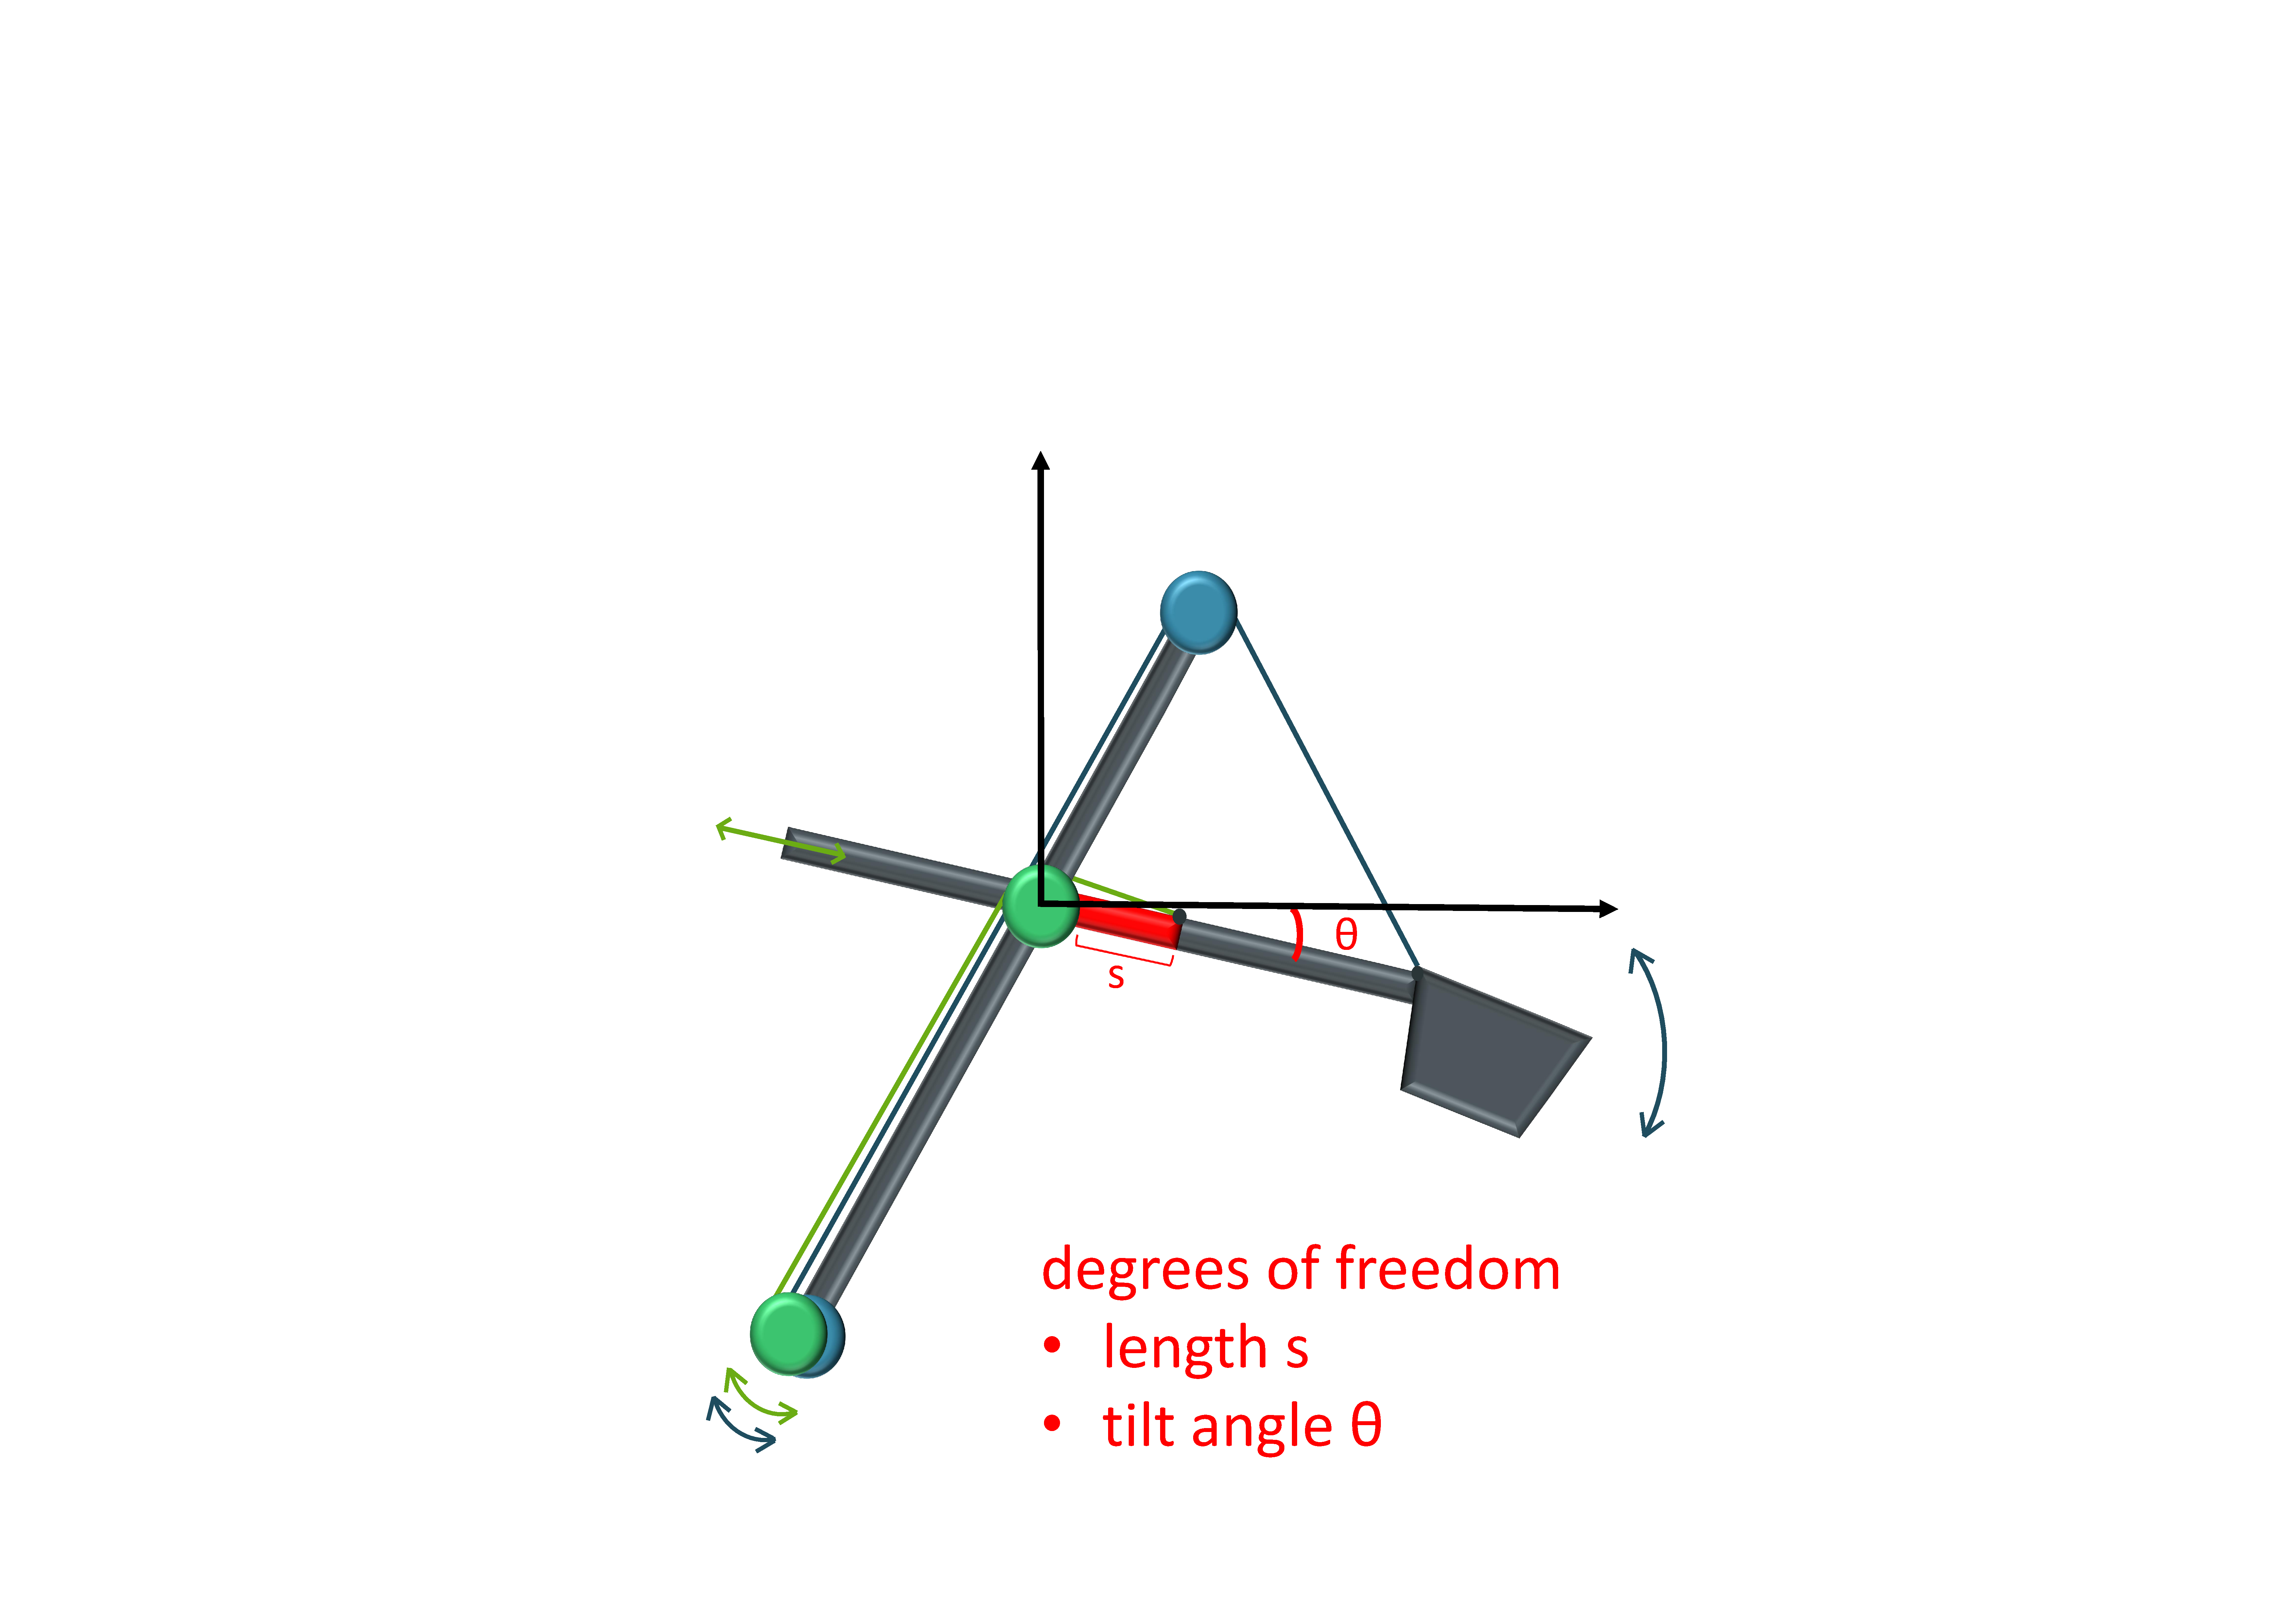
\includegraphics[trim=30cm 5cm 30cm 23cm, clip=true, width=\linewidth]{img/Excavator_dof2}
		\column{.4\linewidth}
			degrees of freedom
			\begin{itemize}
				\item{length $s$}
				\item{tilt angle $\theta$}
			\end{itemize}
	\end{columns}
	
	% s distance between attachment point and upper cable reel of green pulley
	
\end{frame}

\begin{frame}
	\frametitle{Physical Model of Excavator}
	
	%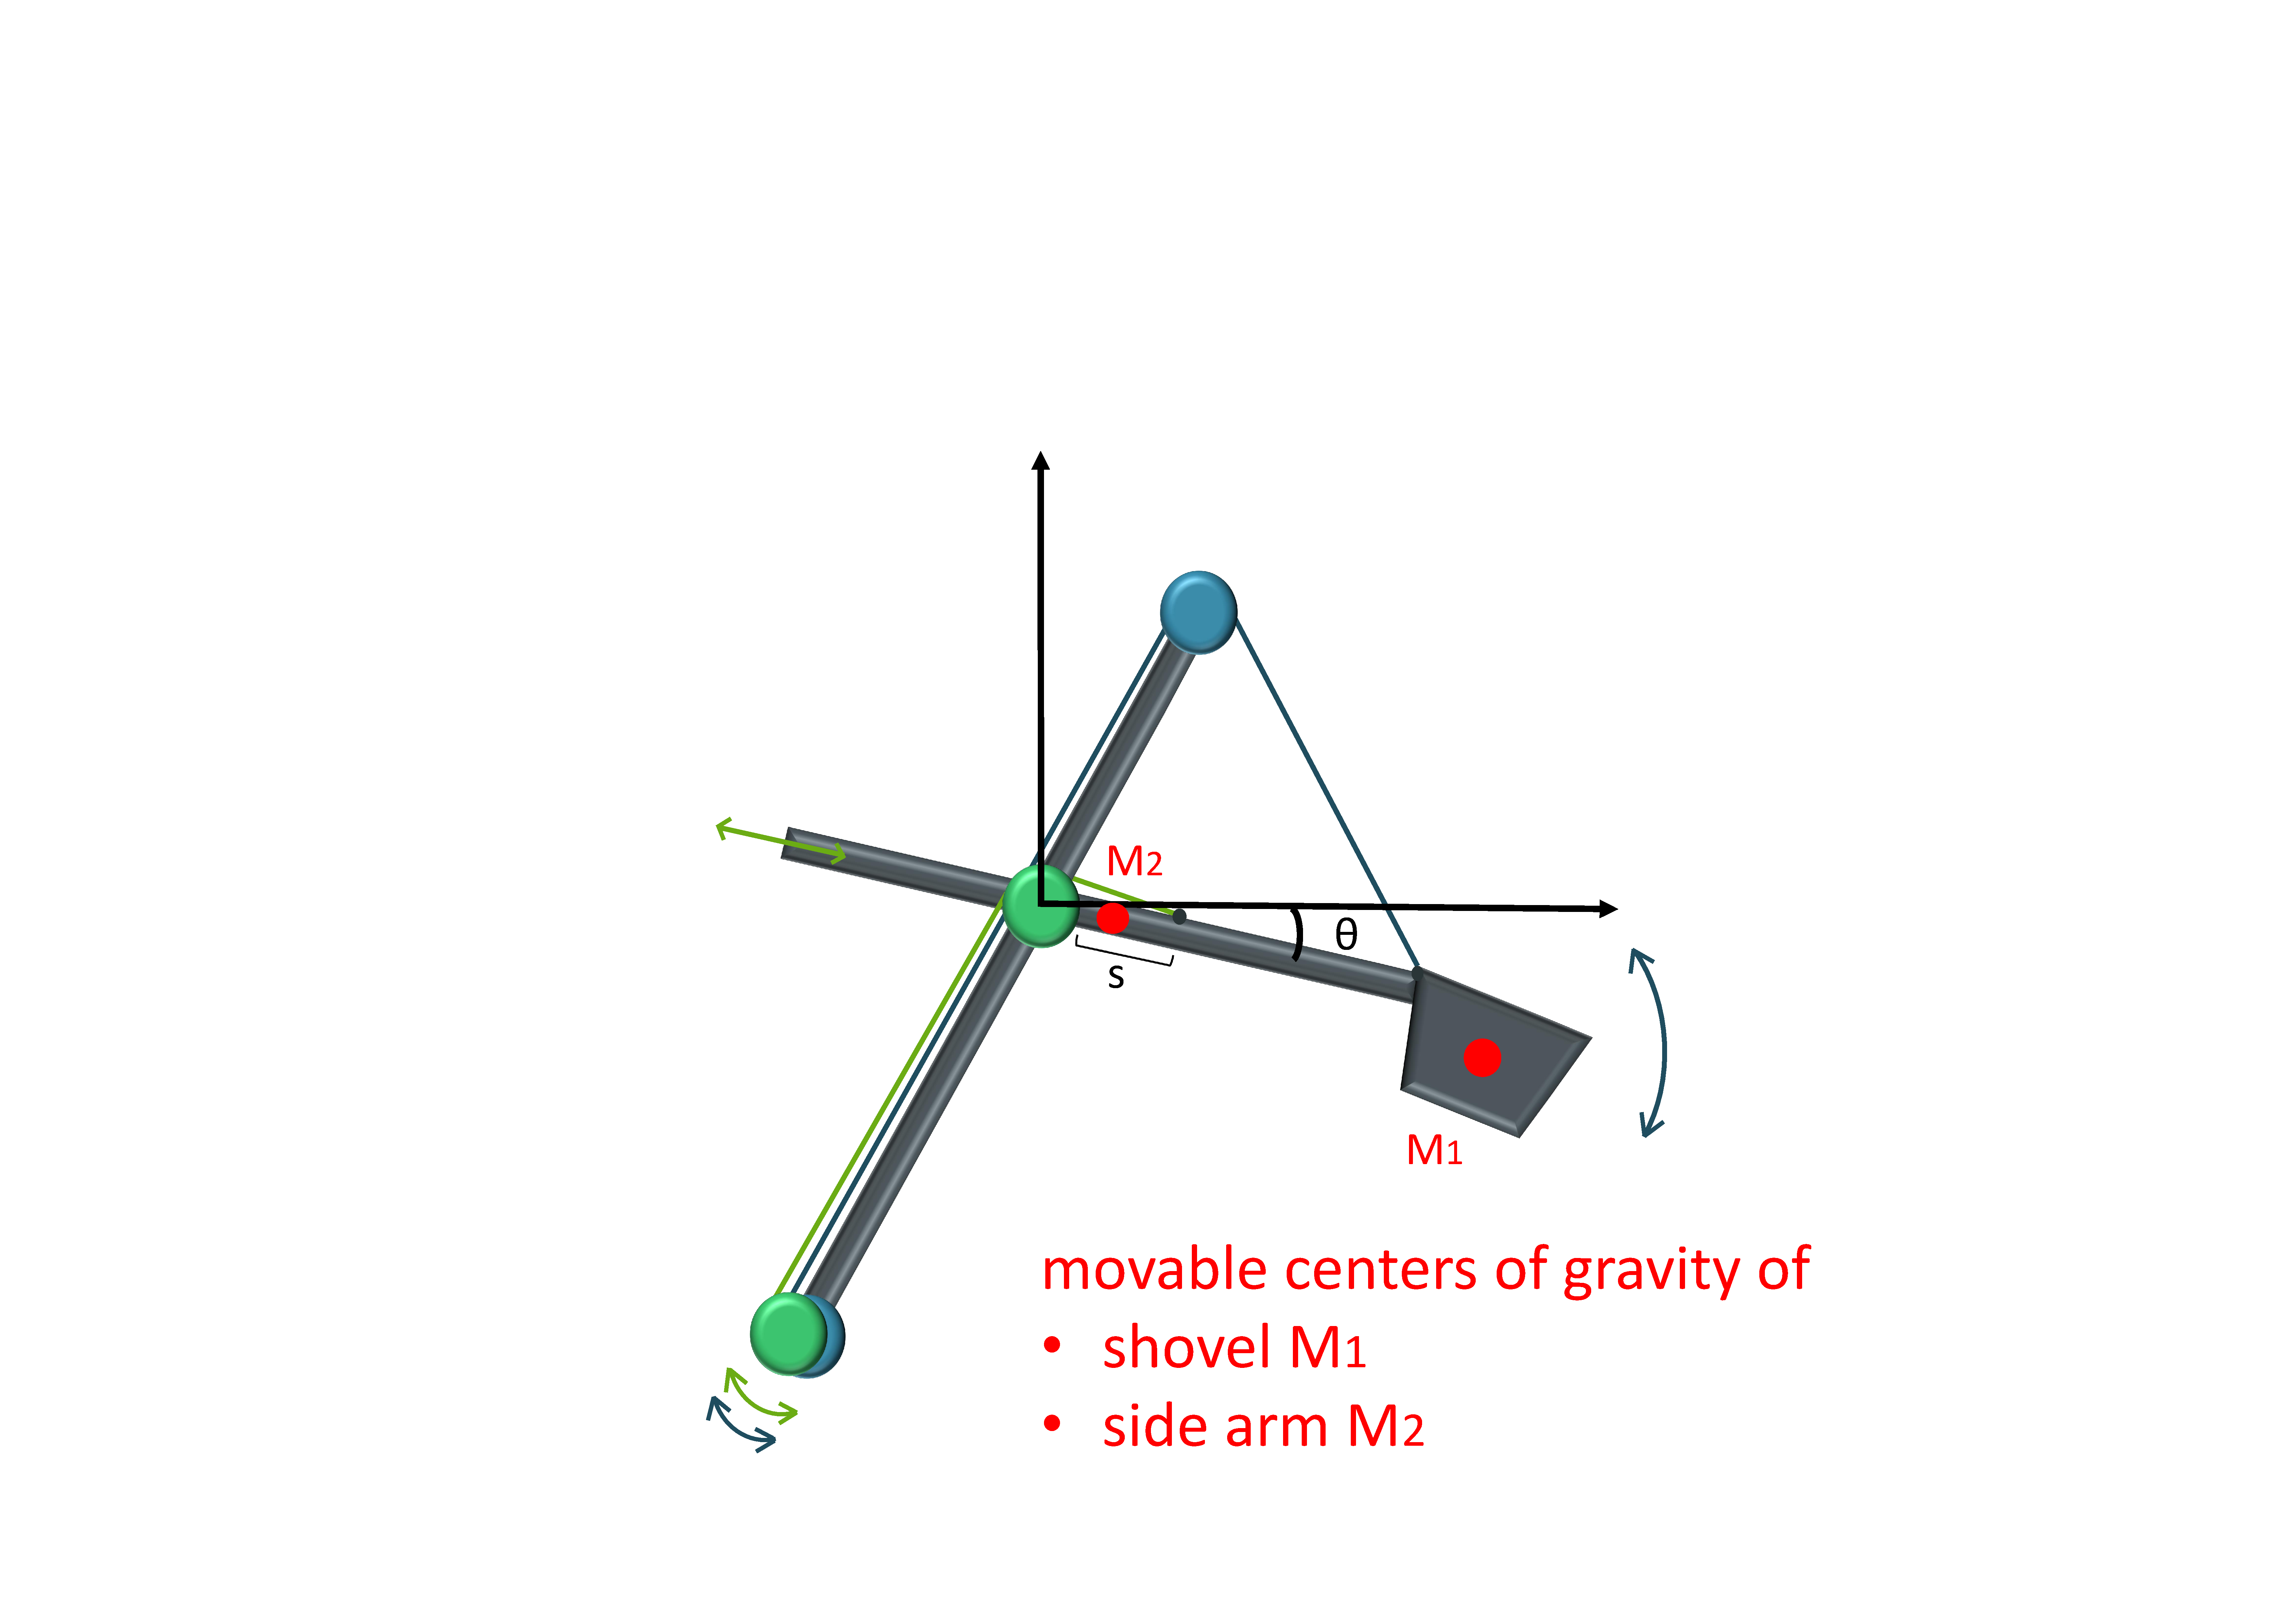
\includegraphics[trim=22cm 5cm 2cm 23cm, clip=true, width=\linewidth]{img/Excavator_mass2}
	
	\begin{columns}
		\column{.6\linewidth}
			\centering
			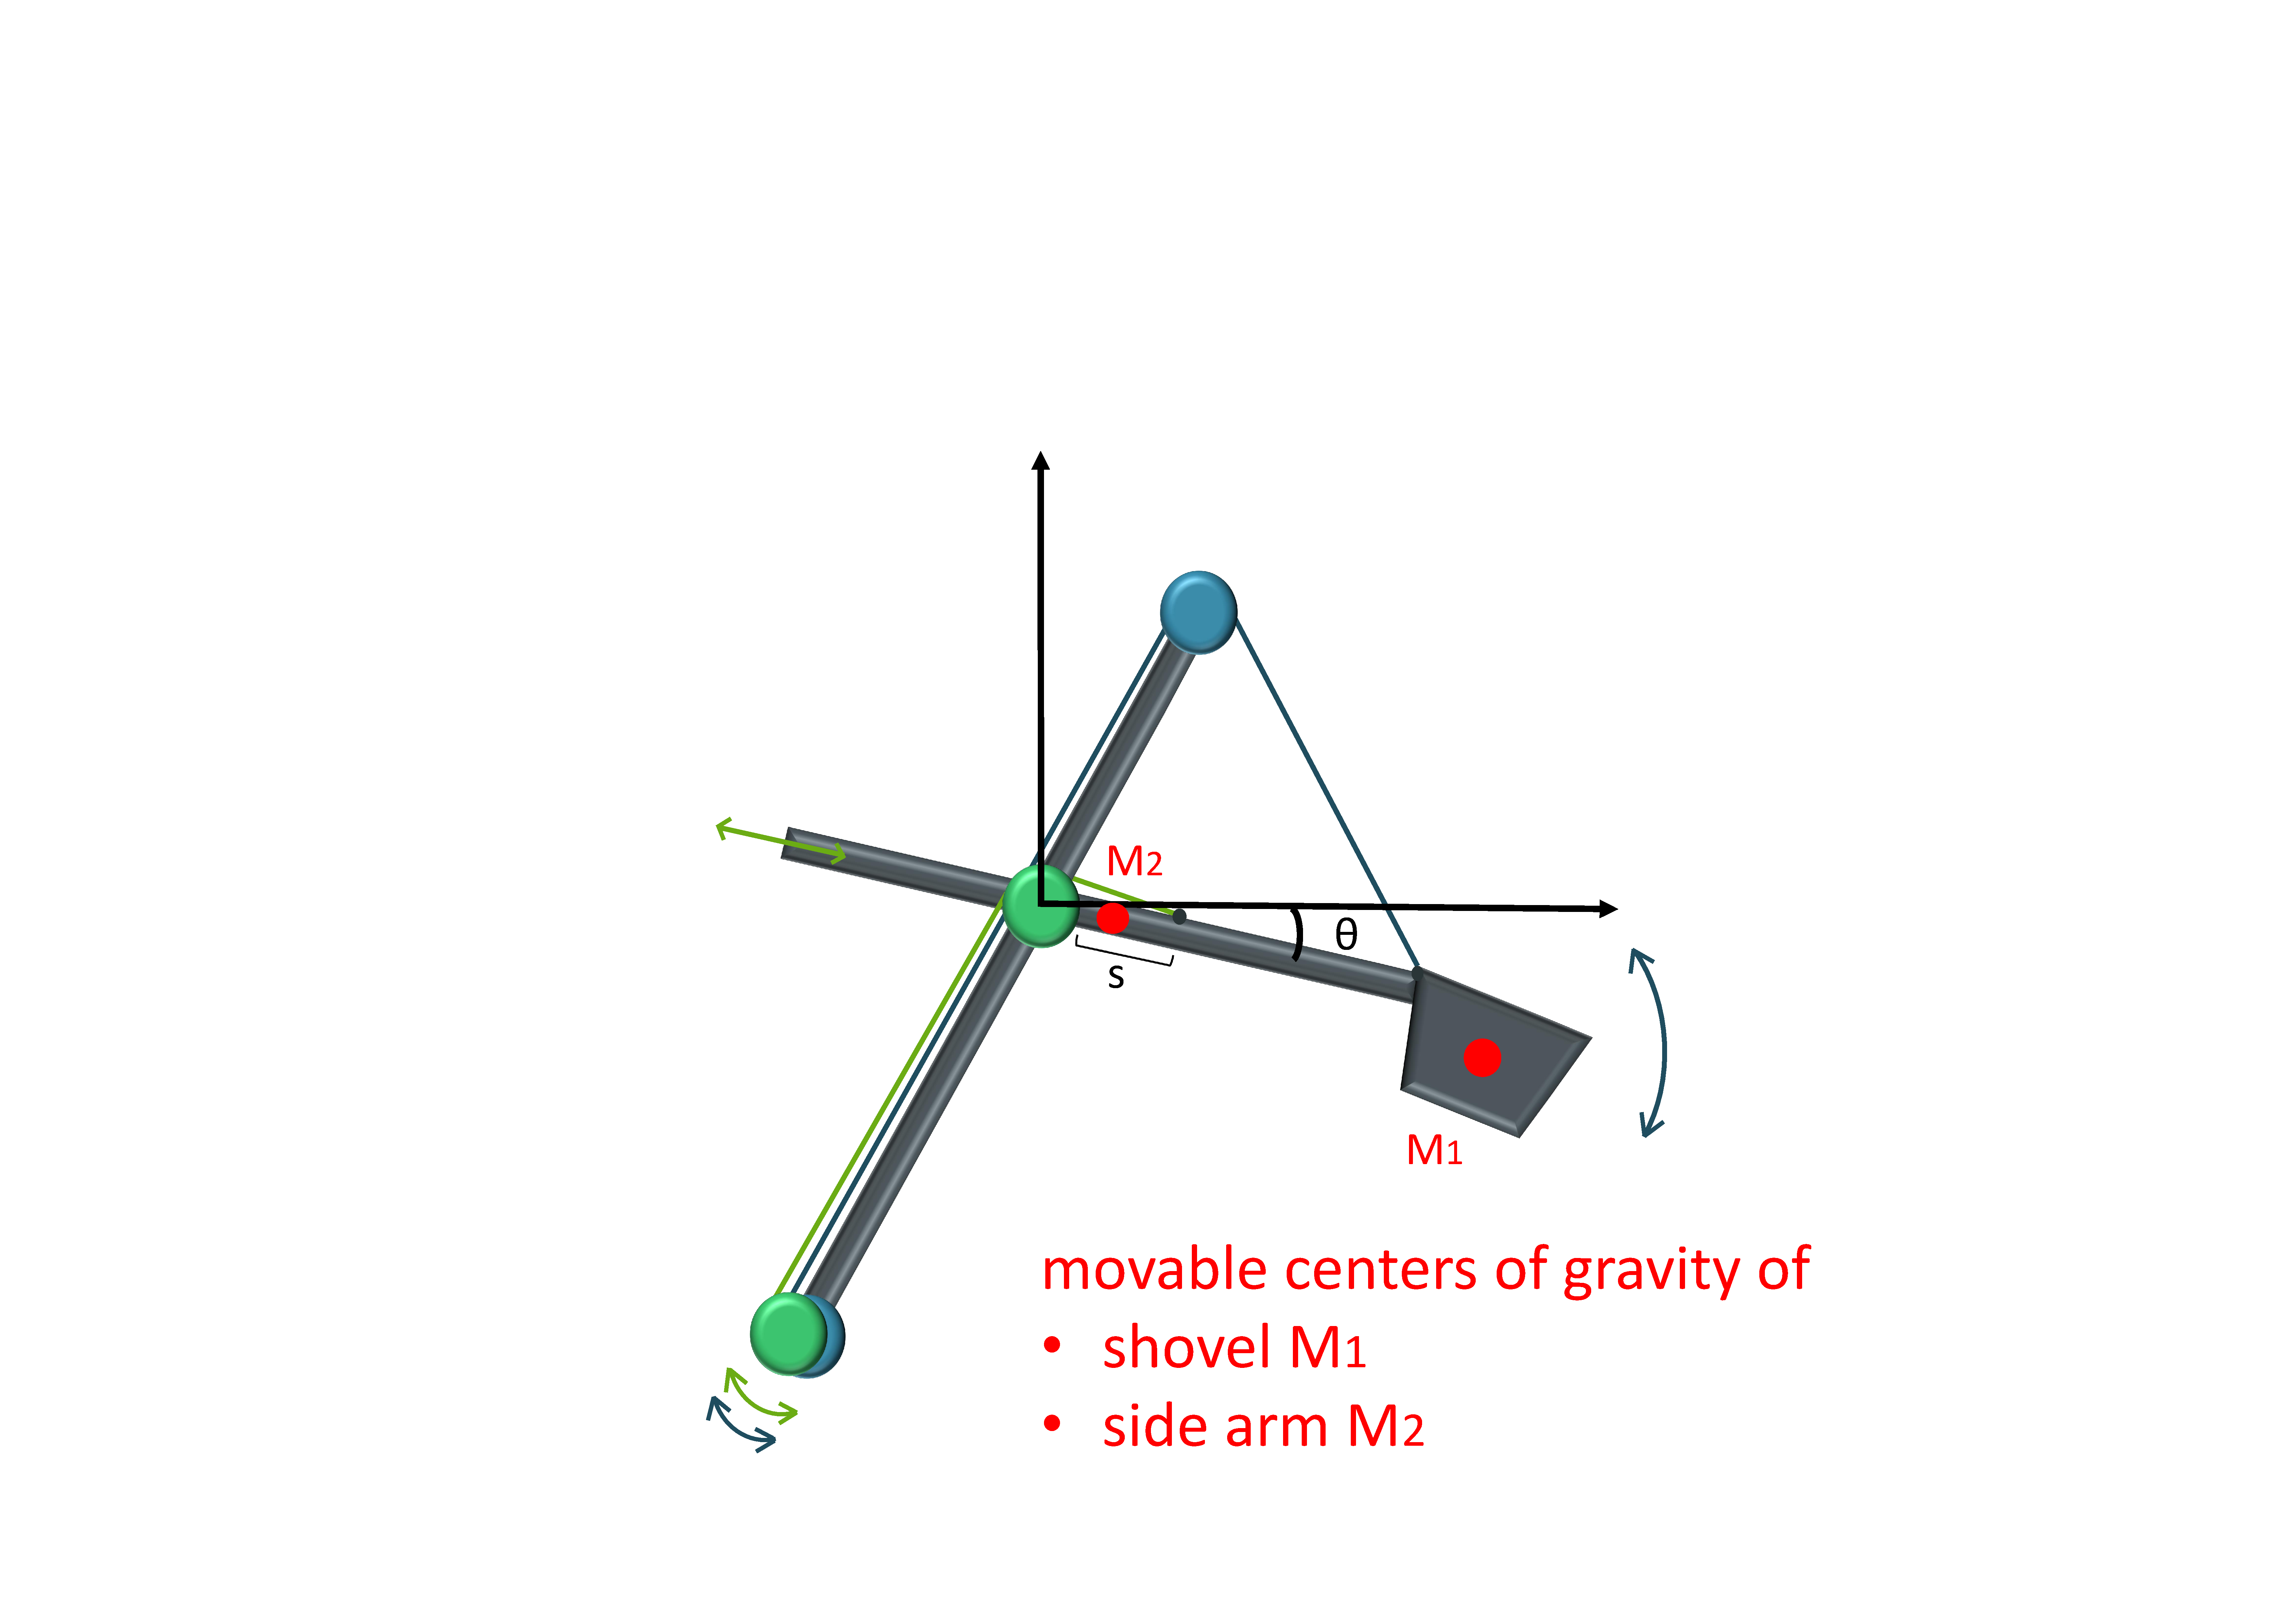
\includegraphics[trim=30cm 5cm 30cm 23cm, clip=true, width=\linewidth]{img/Excavator_mass2}
		\column{.4\linewidth}
			movable centers of gravity of
			\begin{itemize}
				\item{shovel $M_1$}
				\item{arm $M_2$}
			\end{itemize}
	\end{columns}
	
\end{frame}

\begin{frame}
	\frametitle{Physical Model of Excavator}
	
	%where are the point masses? only consider point masses which can be moved i.e. depend on configuration $\rightarrow$ derivative wrt degrees of freedom\\
	%shovel and center of mass of side arm\\
	%other arm is fixed and cant be moved
	
	Assumptions to the model:\\
	$ $ \\
	\begin{itemize}
		\item no mass for the ropes
		\item shovel as point mass % attached on the side arm
		\item no slack/friction between ropes and cable reels
		% ropes and cable reel move with same velocity
		% only bearing friction (friction within cable reels)
	\end{itemize}
	
\end{frame}

%\begin{frame}
	%\frametitle{Kinetic Energy T}
	%
	%Example: energies of $M_2$ 
	%\begin{align*}
		%&E_{\text{kin},M_2} = \frac{1}{2}\ M_2\ \| 
		%v_{O,M_2}(s,\theta,\dot{s},\dot{\theta}) \|^2 \\
		%&E_{\text{rot},M_2} = \frac{1}{2}\ I_{M_2}(s)\ \dot{\theta}^2 \\
	%\end{align*}
	%
	%all kinetic energies:
	%\begin{align*}
	%T\ =\ \ & E_{\text{kin},M_1} + E_{\text{kin},M_2} + E_{\text{rot},M_2}  \\
	%& + E_{\text{rot},B_1} + E_{\text{rot},B_2} + E_{\text{rot},P_1} + E_{\text{rot},P_2} \\
	%\end{align*}
%\end{frame}

%\begin{frame}
	%\frametitle{Potential V}
	%
	%Example: potential of $M_2$
	%\begin{align*}
		%& V_{M_2} = M_2\ g\ h(s,\theta) \\
	%\end{align*}
	%
	%all potentials:
	%\begin{align*}
		%& V = V_{M_1} + V_{M_2} \\
	%\end{align*}
%\end{frame}

%\begin{frame}
	%\frametitle{Involved Forces}
	%\begin{figure}[bth]
	  %\begin{center}
	    %%left, bottom, right, top
	    %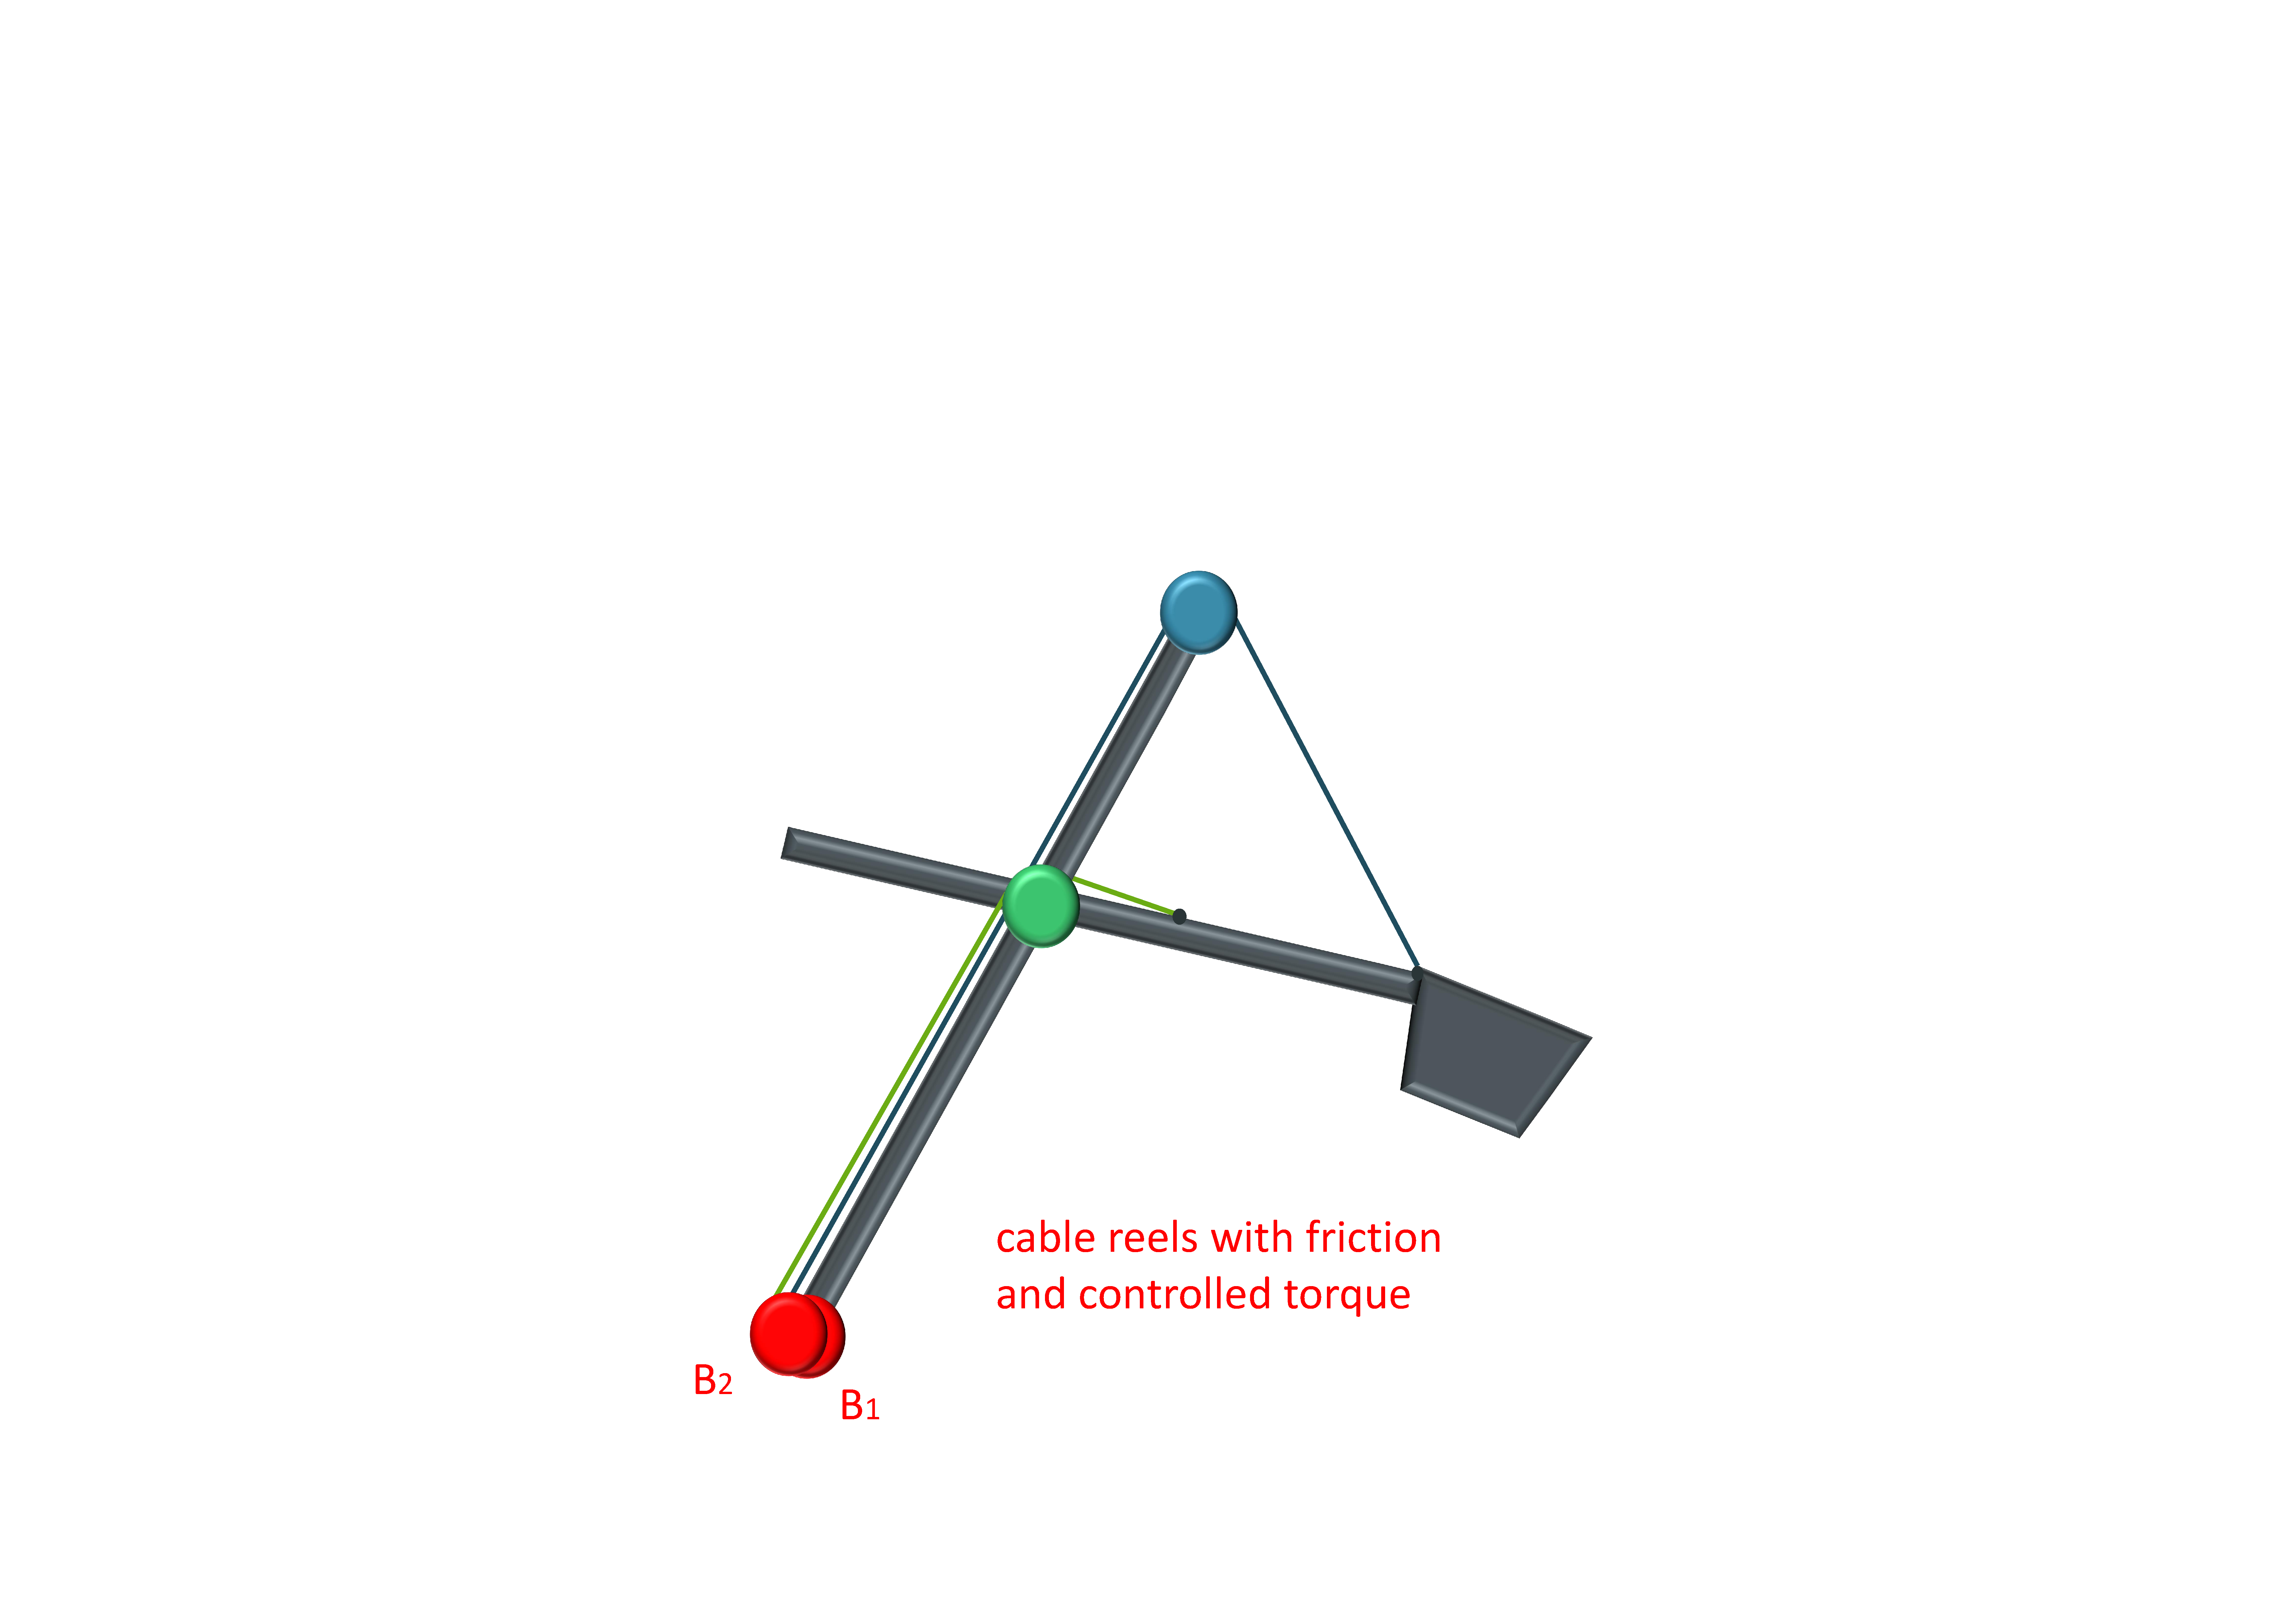
\includegraphics[trim=22cm 5cm 2cm 24cm, clip=true, 
	    %width=\linewidth]{img/Excavator_Only1}
	  %\end{center}
	%\end{figure}
%\end{frame}

\begin{frame}
	\frametitle{Kinetic Energy}
	\begin{columns}
		\column{.6\linewidth}
			\centering
			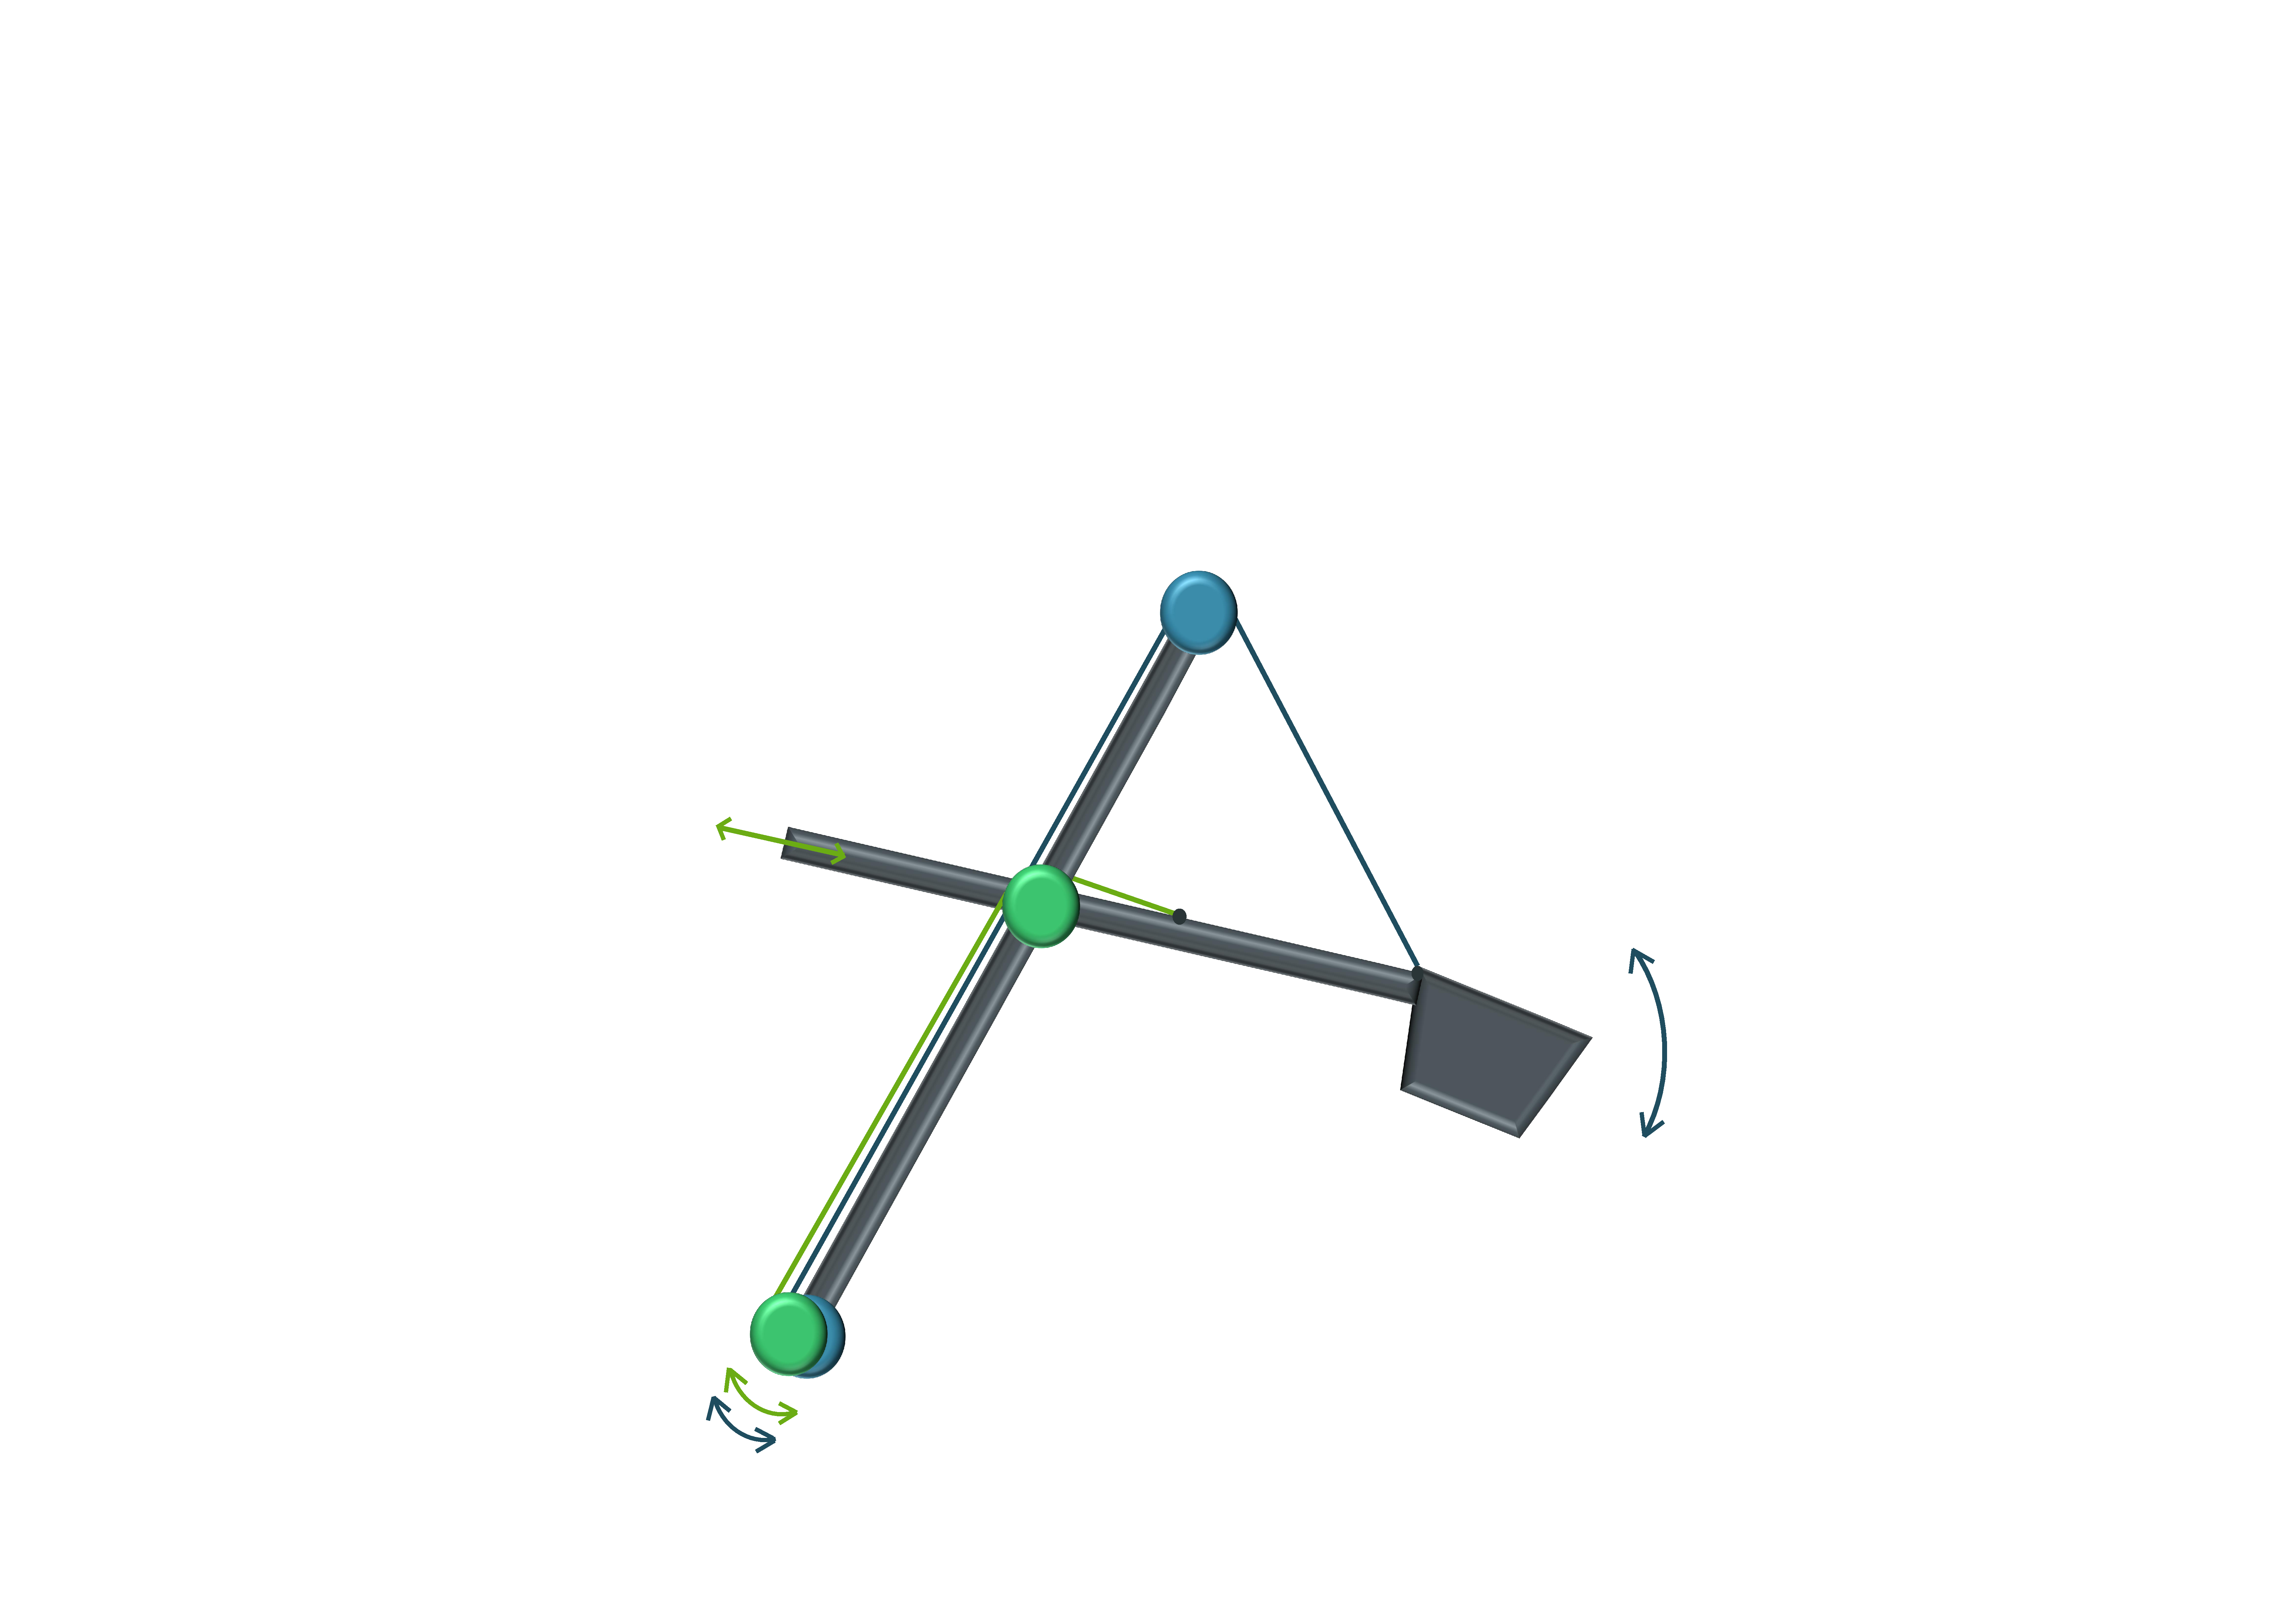
\includegraphics[trim=30cm 5cm 30cm 23cm, clip=true, width=\linewidth]{img/Excavator_Only}
		\column{.4\linewidth}
			\begin{itemize}
				\item{movement of mass}
				\item{rotation of cable reel}
			\end{itemize}
	\end{columns}
\end{frame}

%\begin{frame}
	%\frametitle{Involved Forces}
	%\begin{figure}[bth]
	  %\begin{center}
	    %%left, bottom, right, top
	    %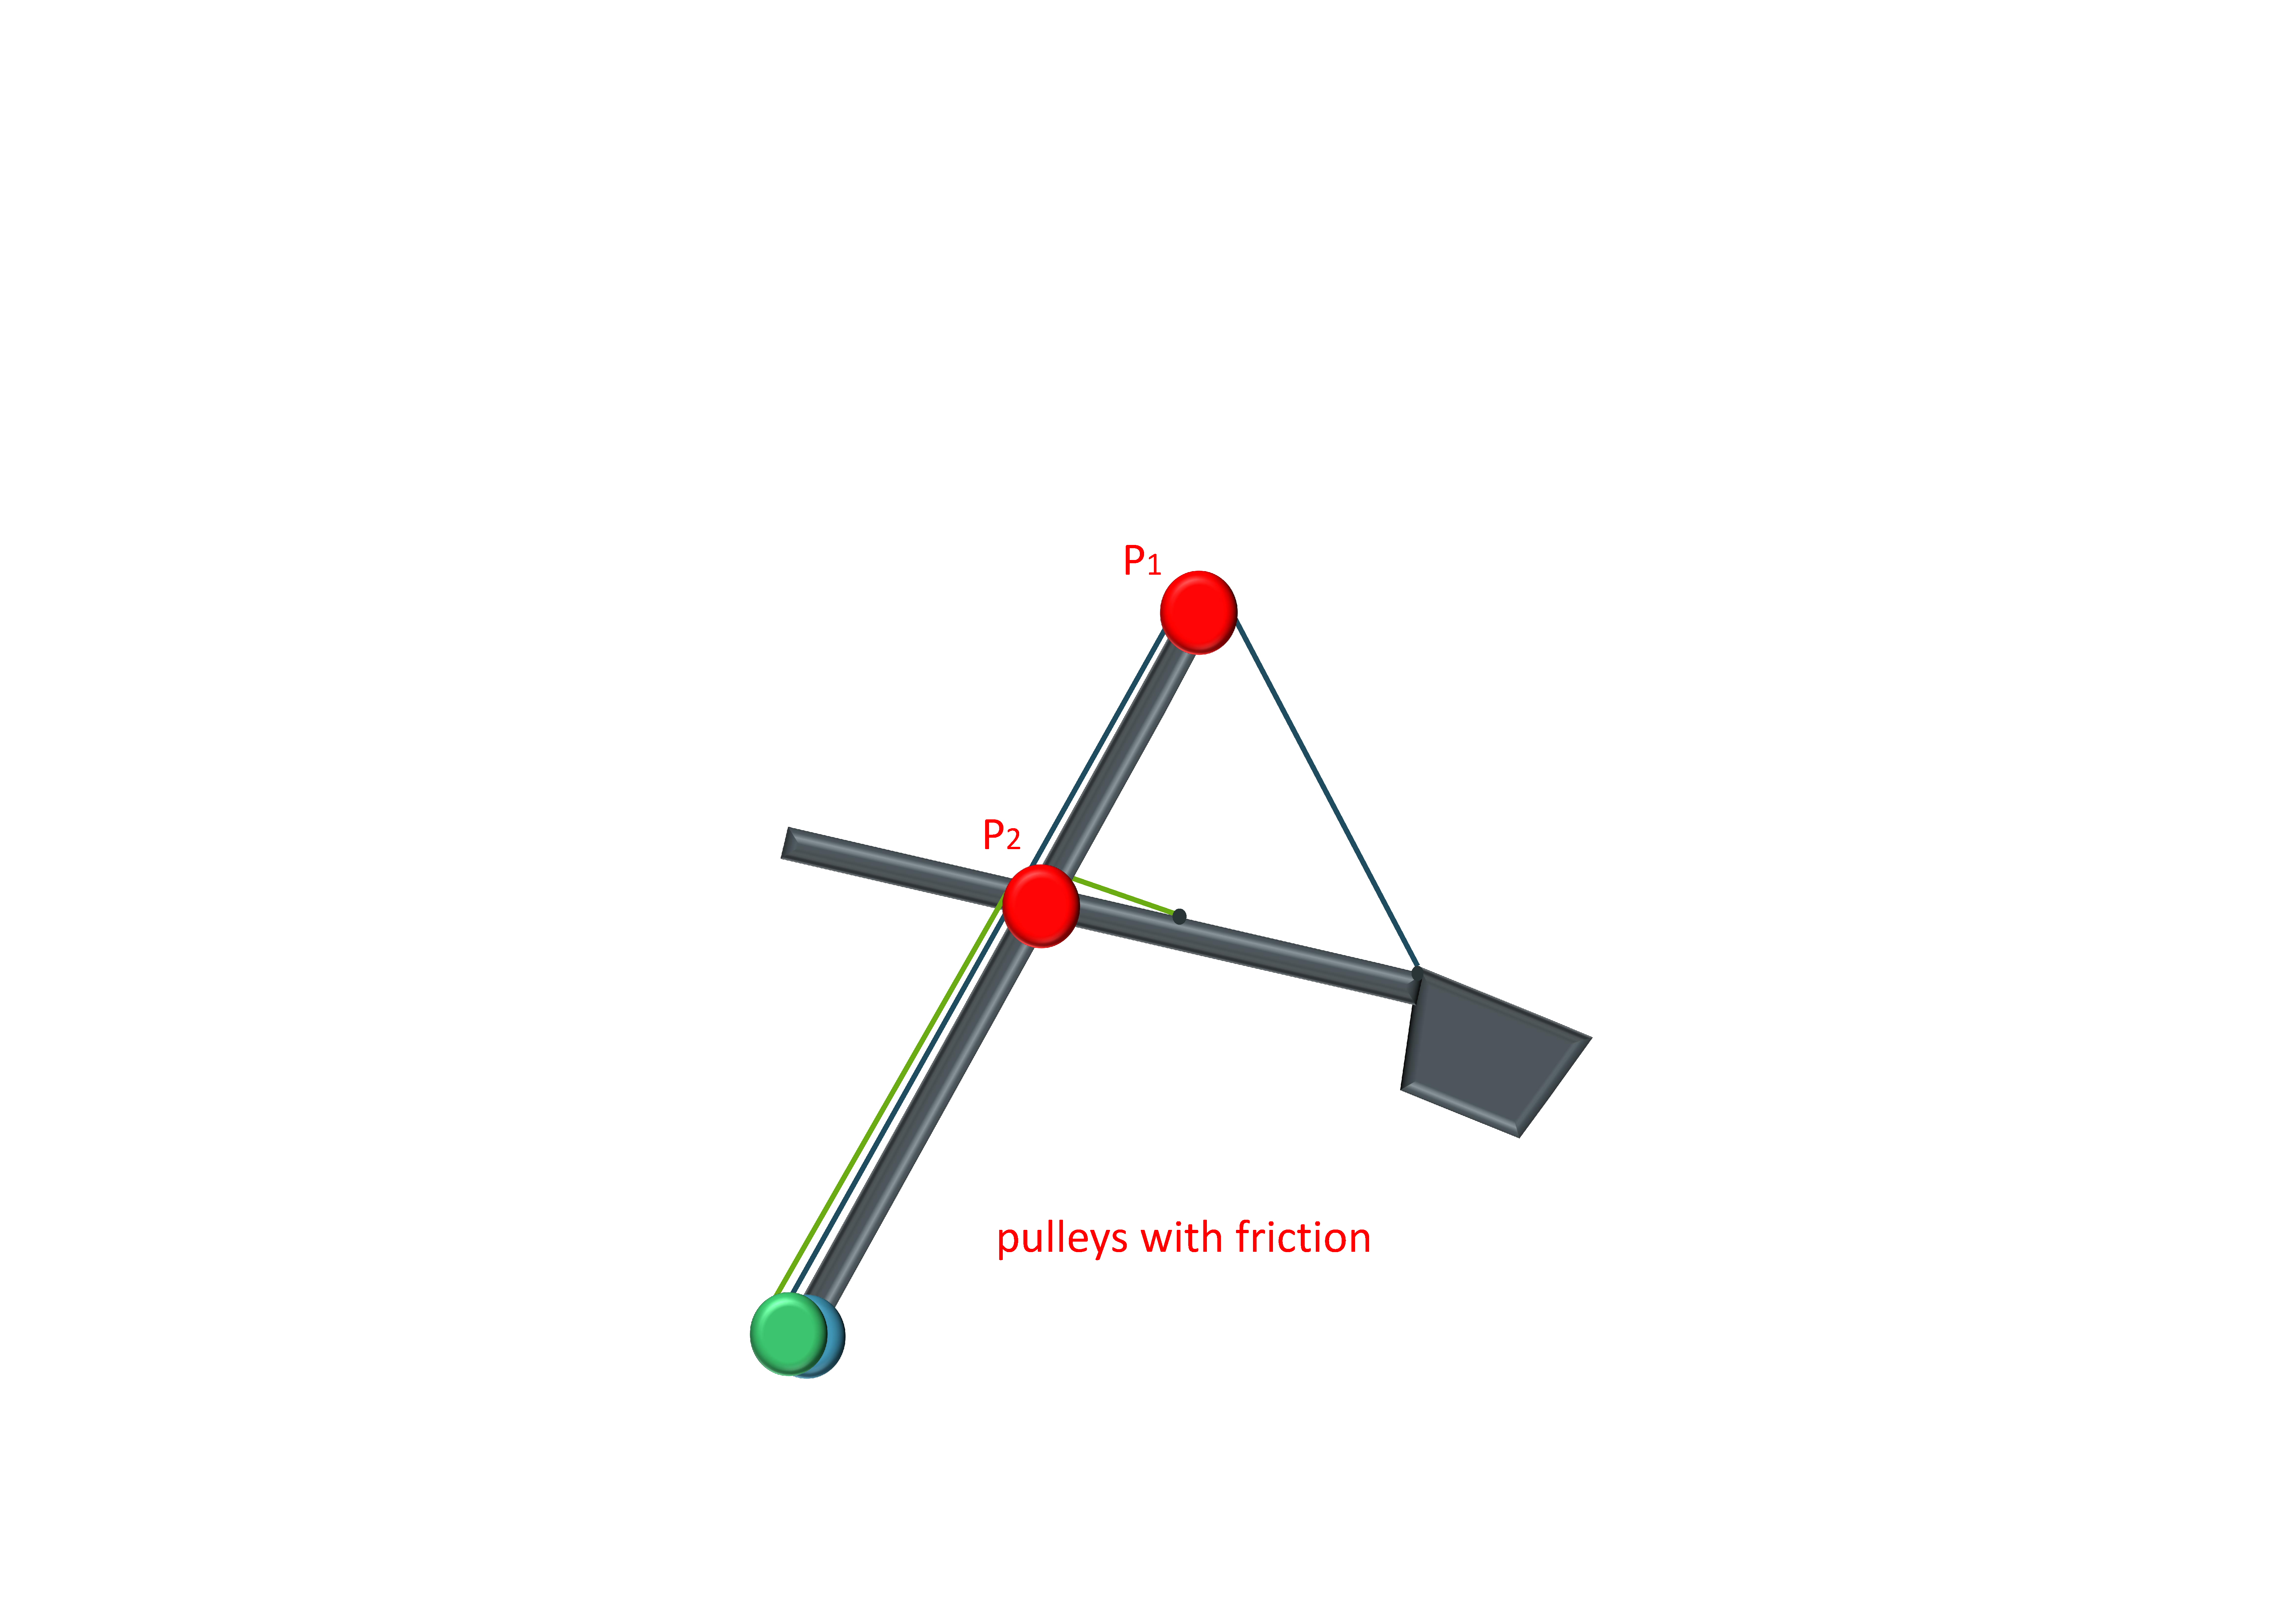
\includegraphics[trim=22cm 5cm 2cm 24cm, clip=true, 
	    %width=\linewidth]{img/Excavator_Only2}
	  %\end{center}
	%\end{figure}
%\end{frame}

\begin{frame}
	\frametitle{Potential Energy}
	\begin{columns}
		\column{.6\linewidth}
			\centering
			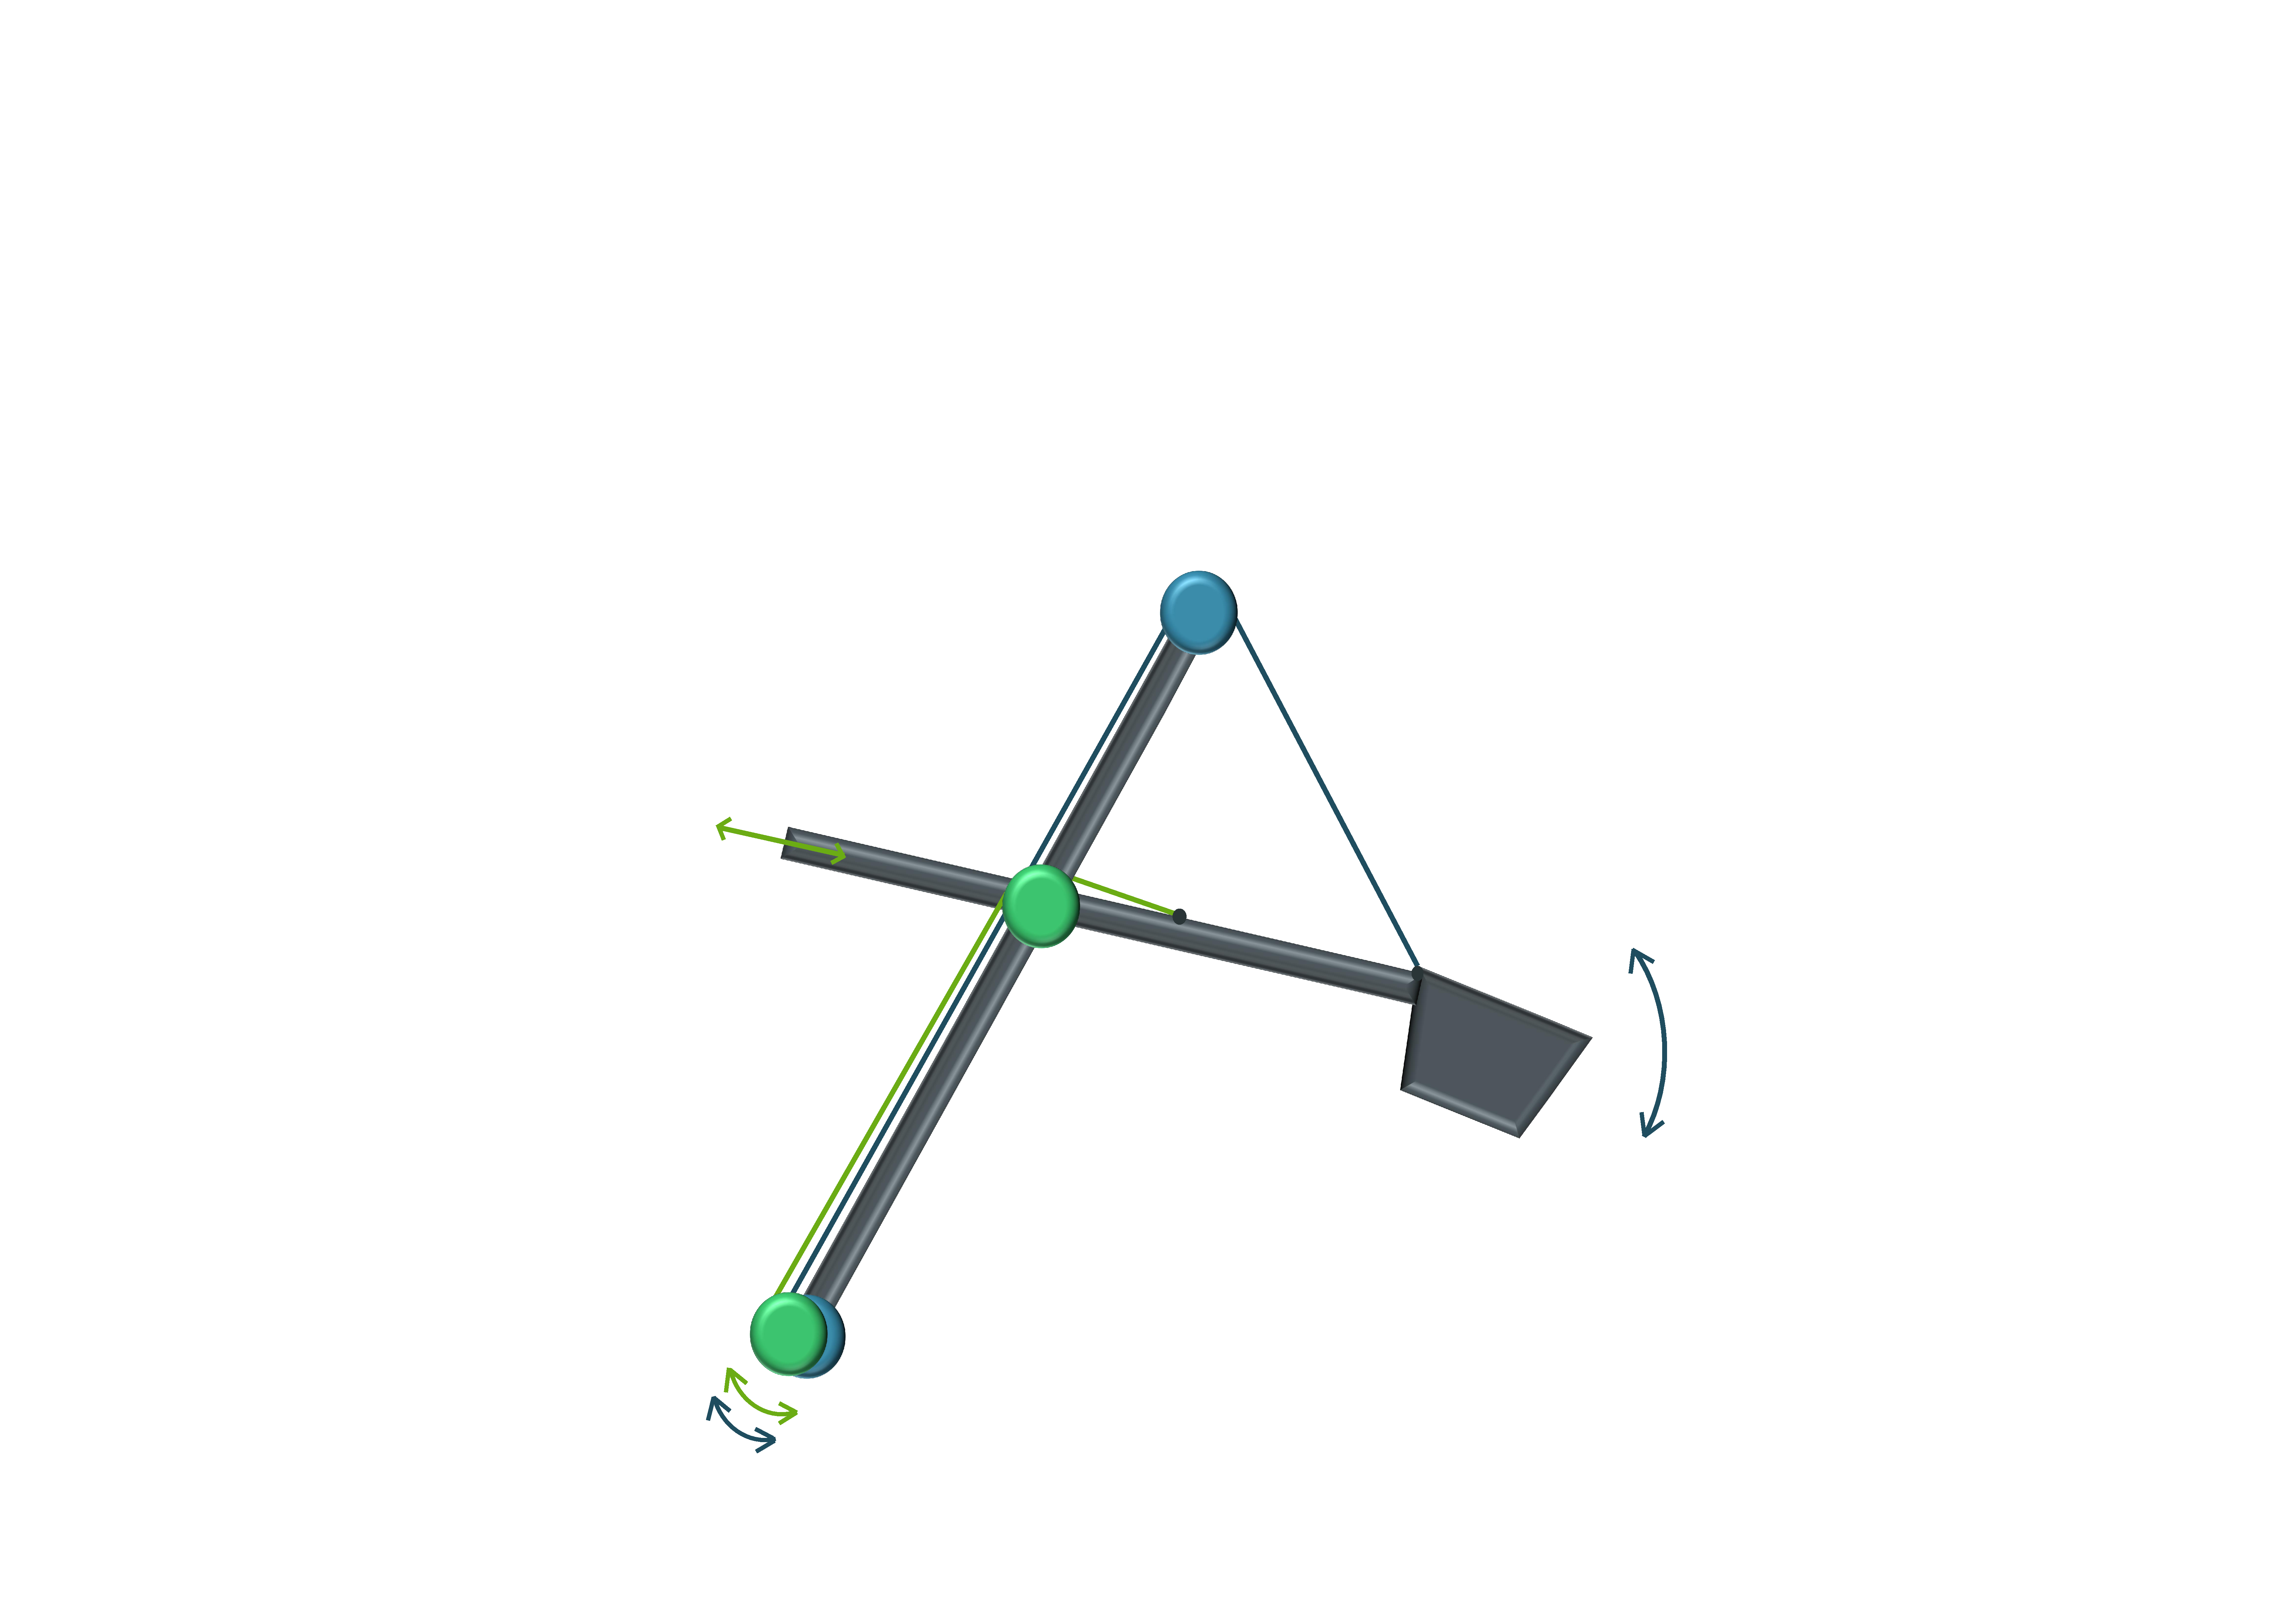
\includegraphics[trim=30cm 5cm 30cm 23cm, clip=true, width=\linewidth]{img/Excavator_Only}
		\column{.4\linewidth}
			gravitational potential energy
	\end{columns}
\end{frame}

%\begin{frame}
	%\frametitle{Involved Forces}
	%\begin{figure}[bth]
	  %\begin{center}
	    %%left, bottom, right, top
	    %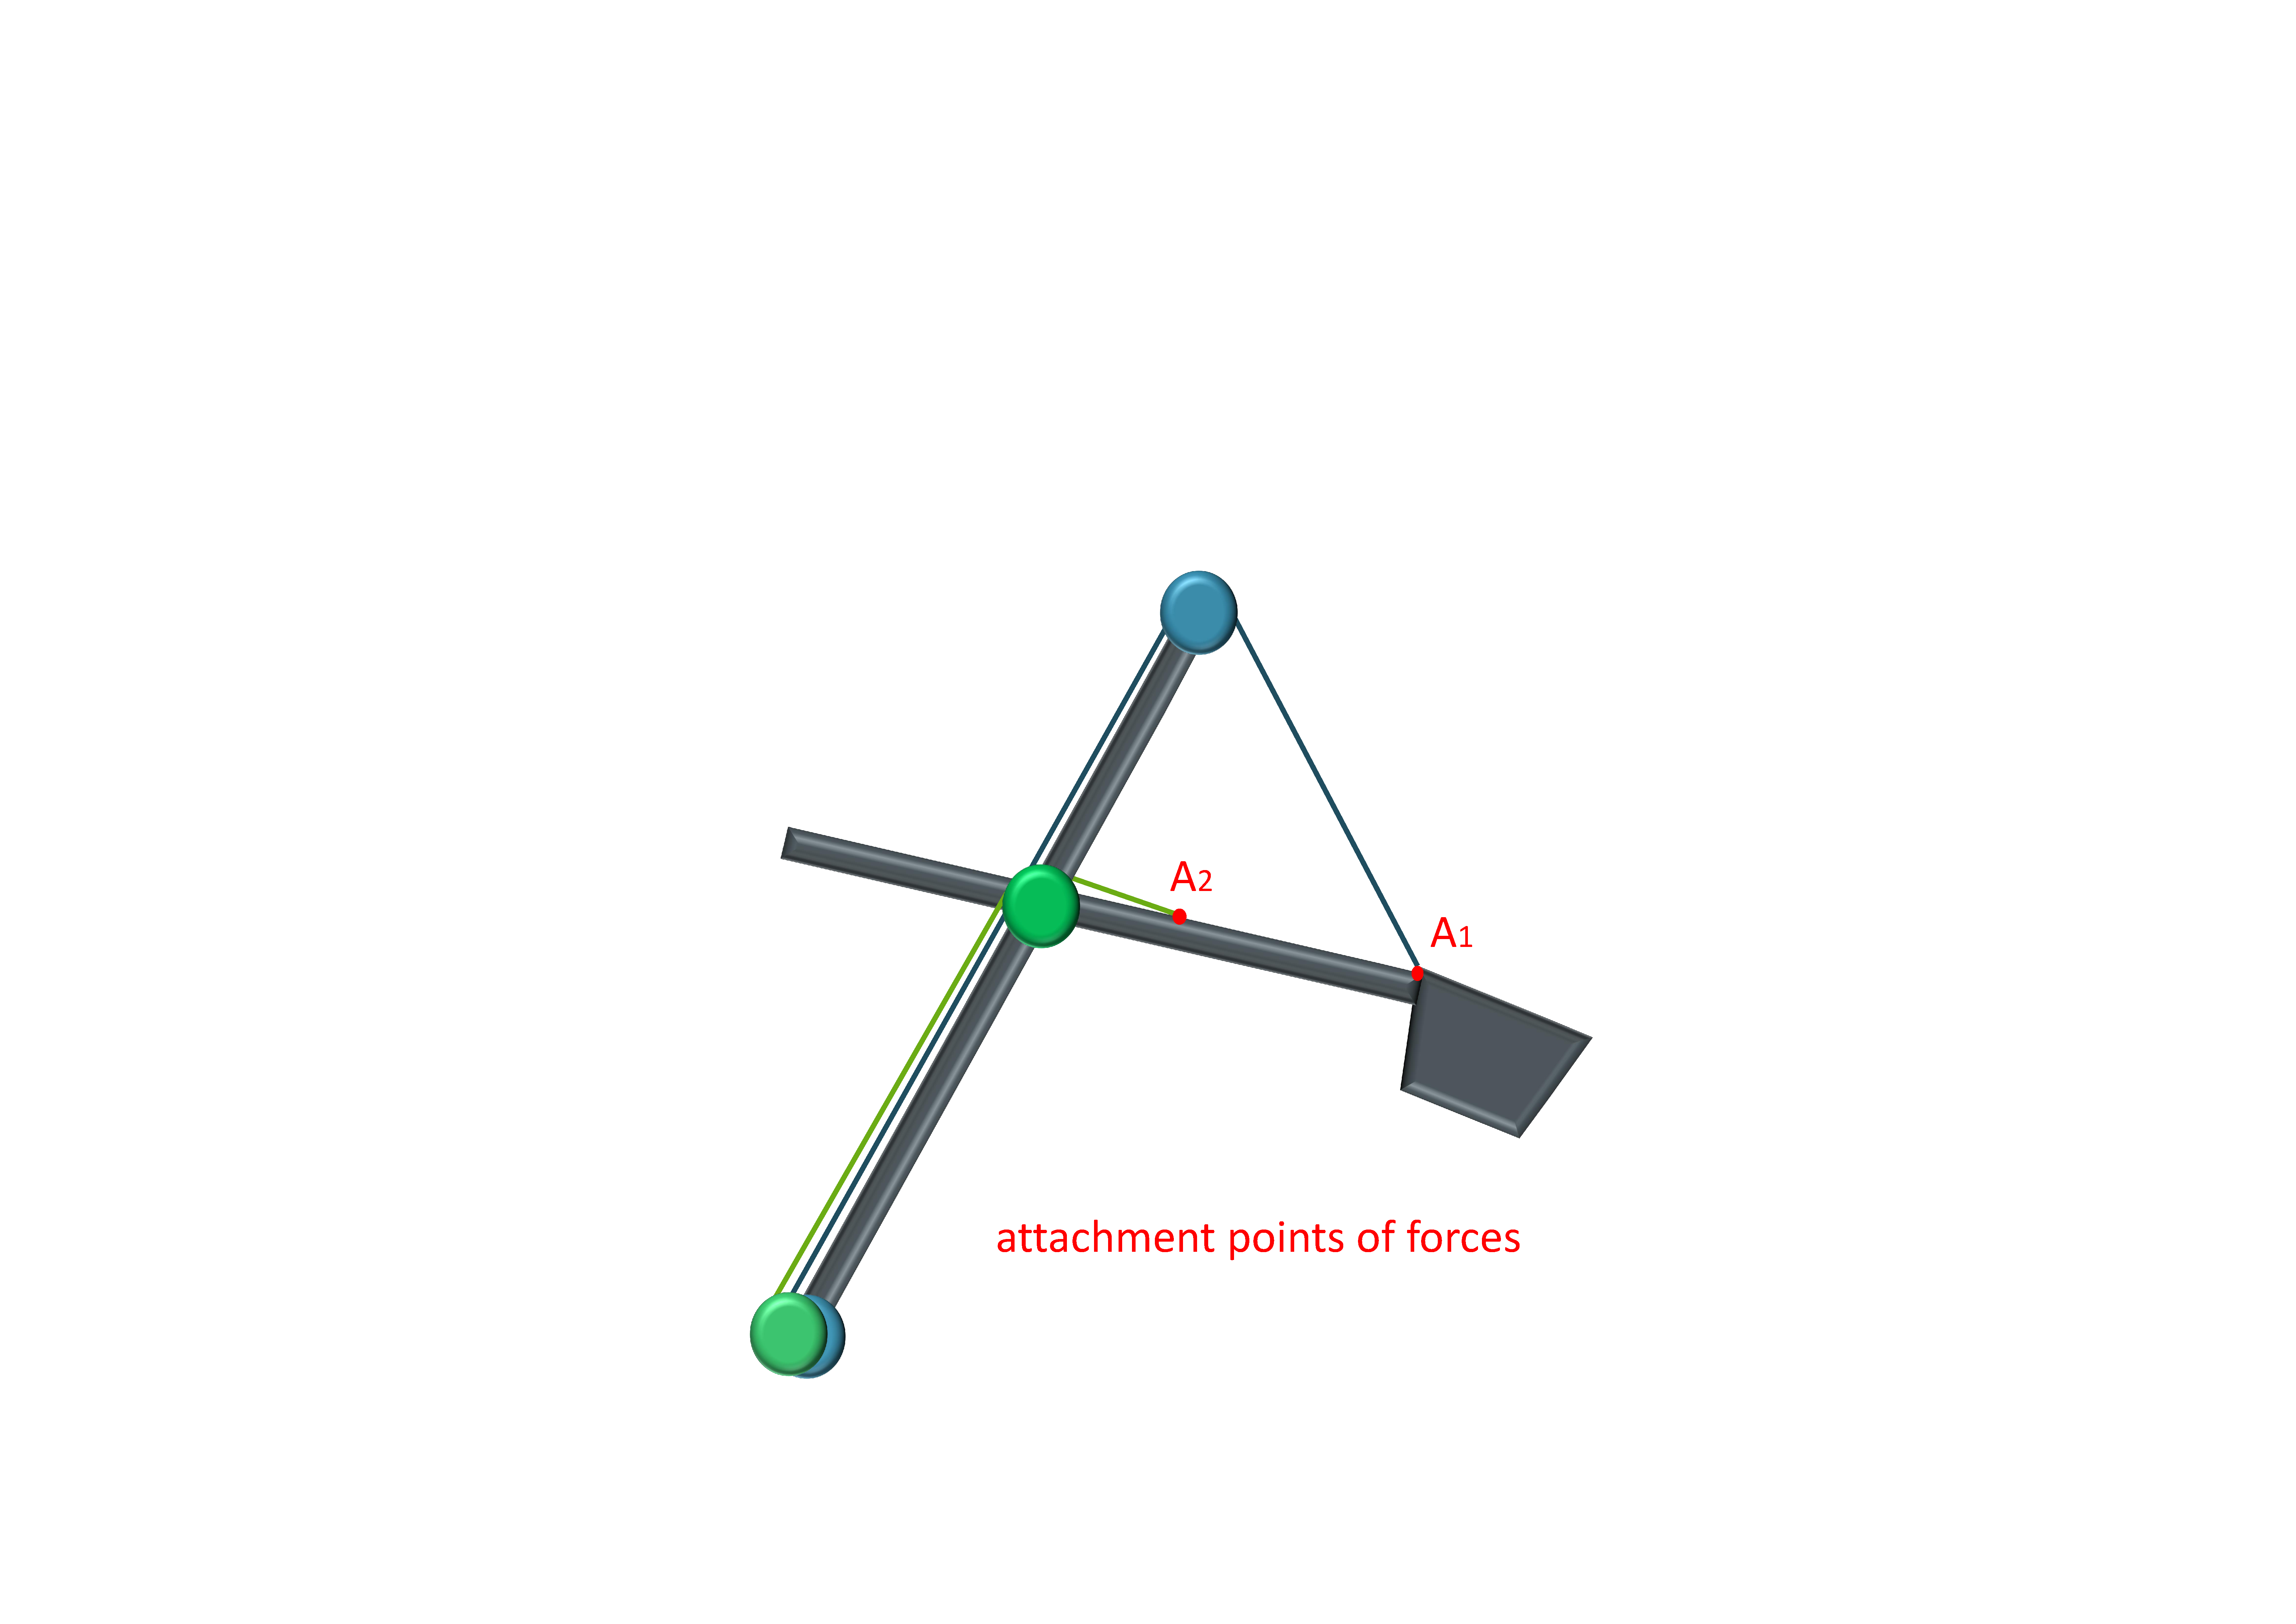
\includegraphics[trim=22cm 5cm 2cm 24cm, clip=true, 
	    %width=\linewidth]{img/Excavator_Only3}
	  %\end{center}
	%\end{figure}
%\end{frame}

\begin{frame}
	\frametitle{Generalized Forces}
	\begin{columns}
		\column{.6\linewidth}
			\centering
			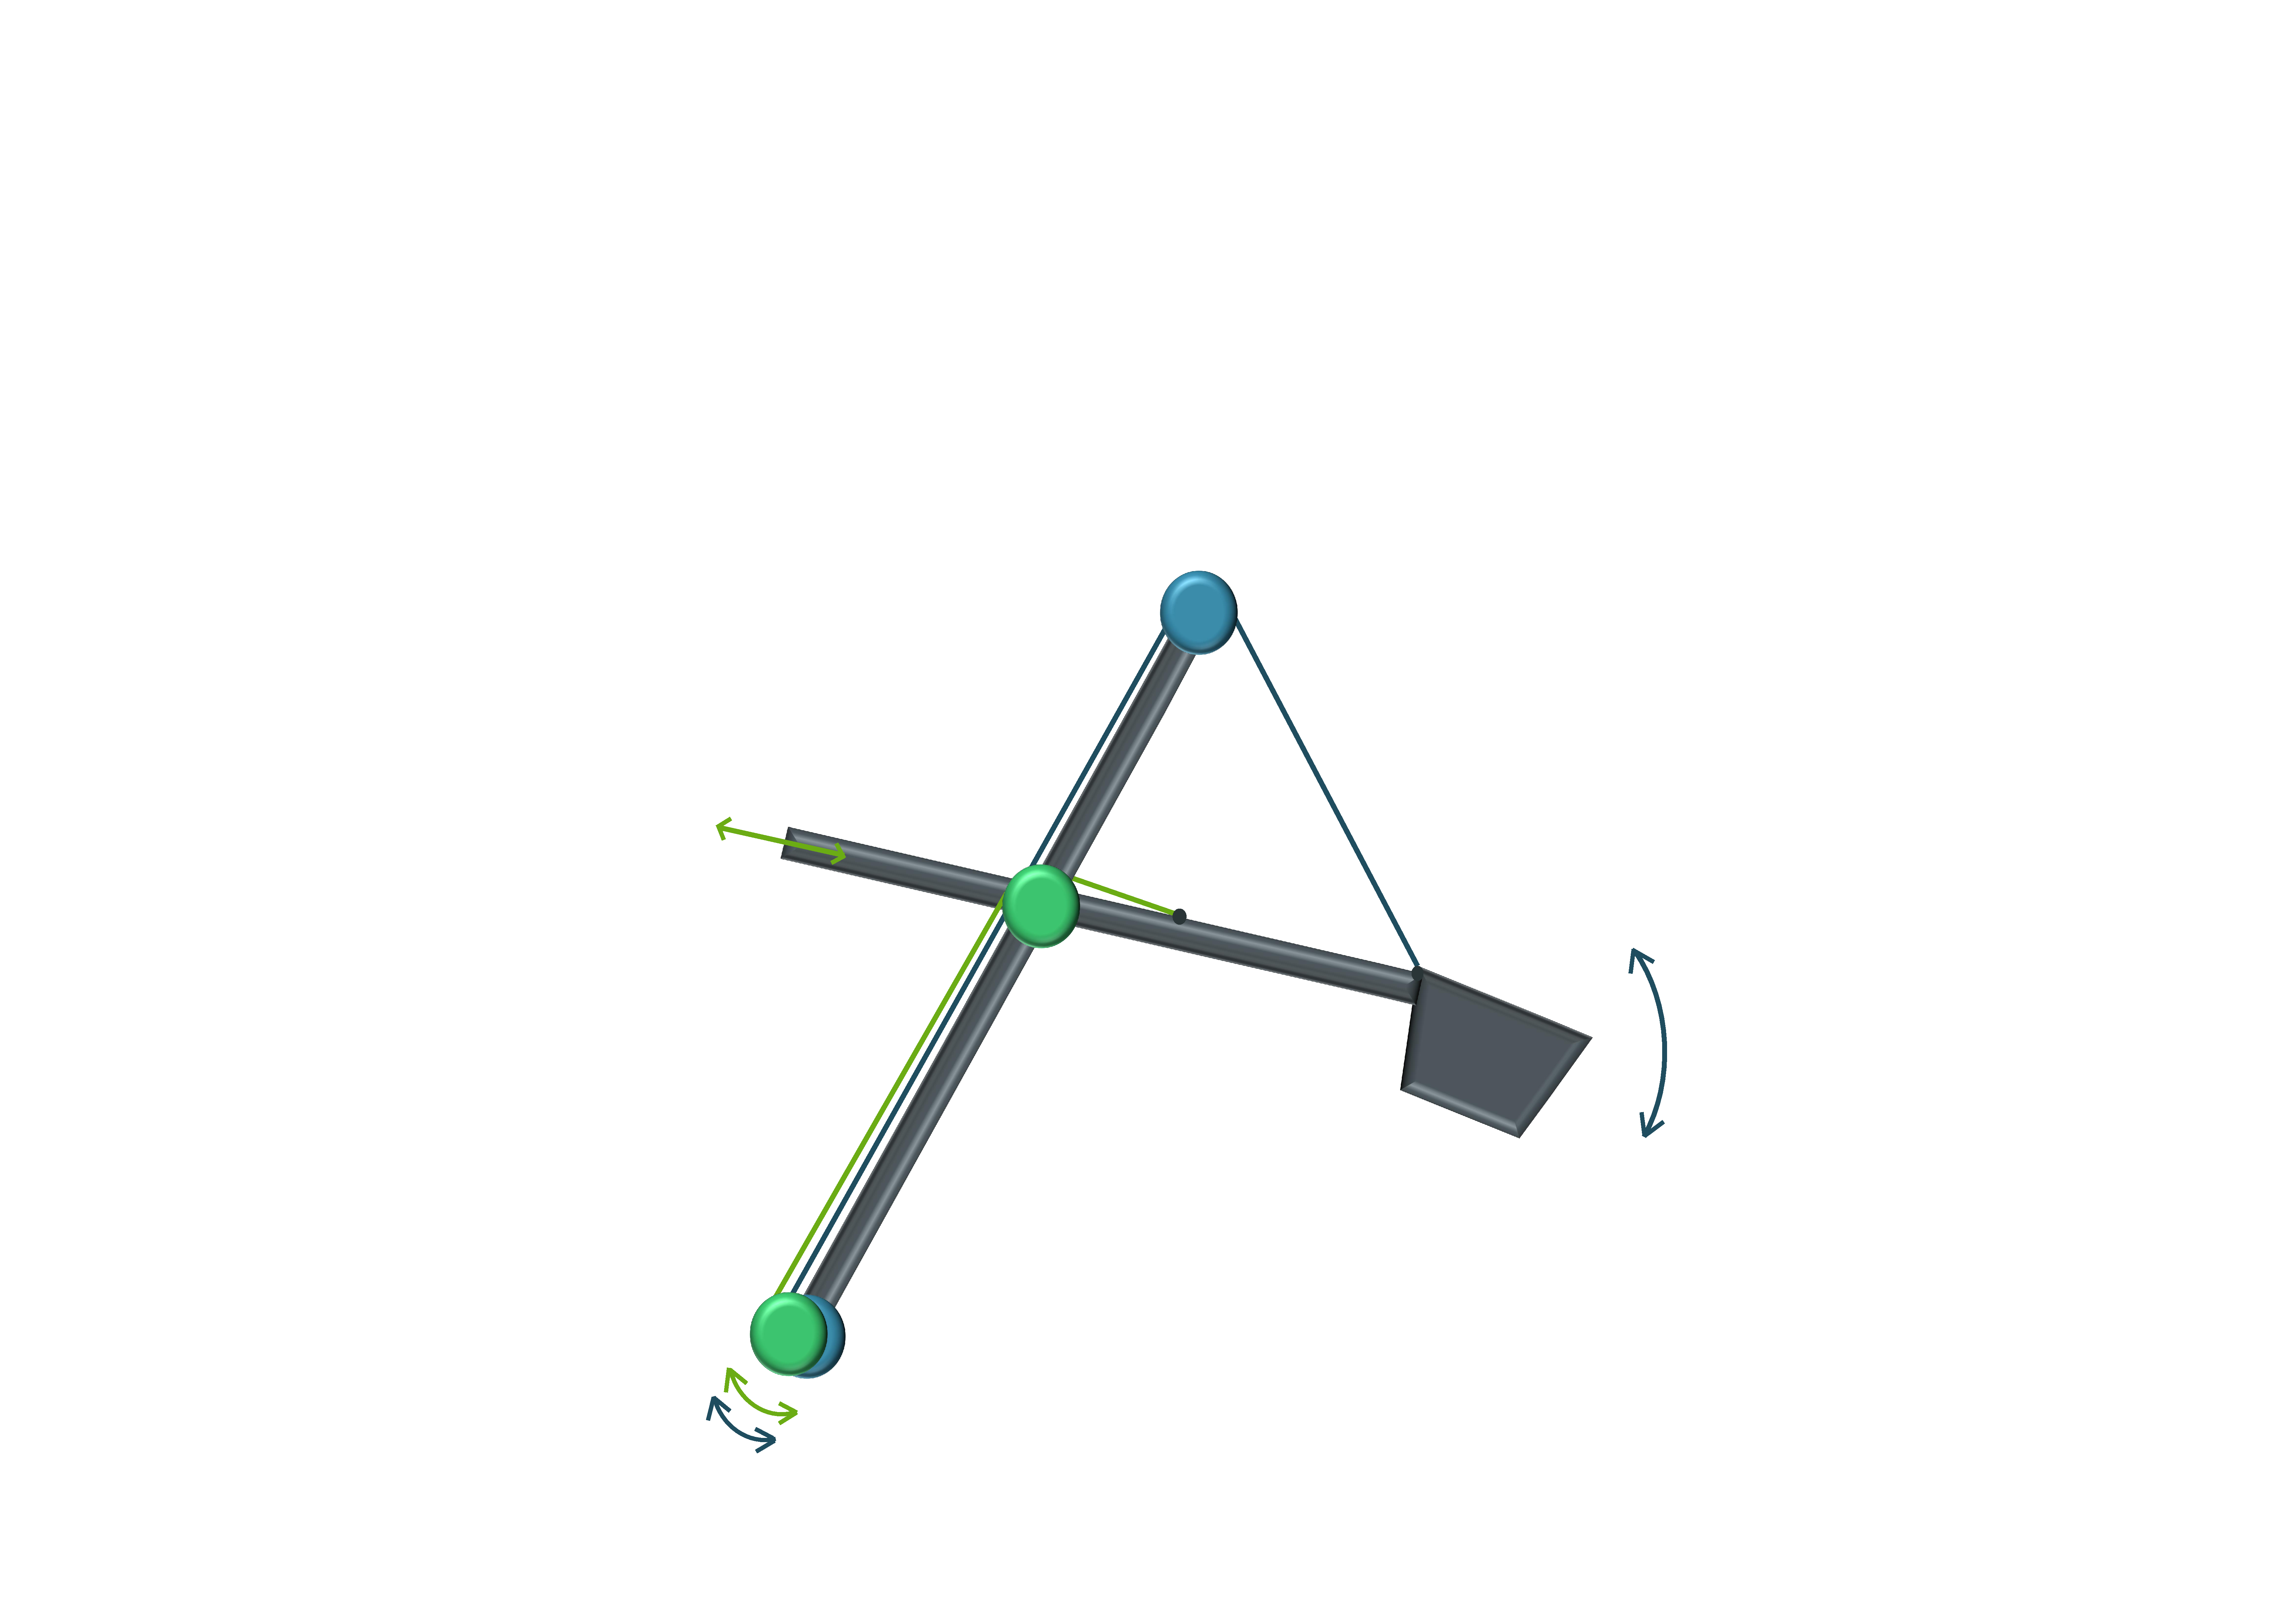
\includegraphics[trim=30cm 5cm 30cm 23cm, clip=true, width=\linewidth]{img/Excavator_Only}
		\column{.4\linewidth}
			\begin{itemize}
				\item{torque on cable reel}
				\item{friction of cable reel}
			\end{itemize}
	\end{columns}
\end{frame}

%\begin{frame}
	%\frametitle{Generalized Forces Q}
	%
	%Example: force at $A_2$:
	%\begin{align*}
	  %&F_{A_2} = \left[ \frac{\tau_{B_2}}{r_{B_2}} - \mu_{B_2} 
	  %\frac{\dot{s}}{r_{B_2}} - \mu_{P_2} \frac{\dot{s}}{r_{P_2}} \right]
	  %\left(
	  %\begin{matrix}
	    %\cos(\theta) \\
	    %\sin(\theta) \\
	  %\end{matrix}
	  %\right) \\
	%\end{align*}
	%
	%all generalized forces:
	%\begin{align*}
	  %&Q_s = \left( \frac{\partial r_{A_1}}{\partial s} \right)^T F_{A_1} 
	  %+ \left( \frac{\partial r_{A_2}}{\partial s} \right)^T F_{A_2} \\
	  %&Q_{\theta} = \left( \frac{\partial r_{A_1}}{\partial \theta} 
	  %\right)^T F_{A_1} + \left( \frac{\partial r_{A_2}}{\partial \theta} 
	  %\right)^T F_{A_2} \\
	%\end{align*}
%\end{frame}

%\begin{frame}
	%\frametitle{Parameters}
	%
	%\begin{tabular}{ll}
	  %& \\
	  %masses & $M_1$, $M_2$ \\
	  %&\\
	  %inertia of pulleys & $I_{B_1}$, $I_{B_2}$, $I_{P_1}$, $I_{P_2}$ \\
	  %&\\
	  %friction coefficients & $\mu_{B_1}$, $\mu_{B_2}$, $\mu_{P_1}$, 
	  %$\mu_{P_2}$  \\
	%\end{tabular}
%\end{frame}

\begin{frame}
	\frametitle{Lagrange Formalism}
	
	\begin{align*}
	  &\frac{d}{dt}\left(\frac{\partial T}{\partial \dot{s}}\right) -
	  \frac{\partial T}{\partial s} +
	  \frac{\partial V}{\partial s}
	  = Q_s \\
	  &{}\\
	  &\frac{d}{dt}\left(\frac{\partial T}{\partial \dot{\theta}}\right) -
	  \frac{\partial T}{\partial \theta} +
	  \frac{\partial V}{\partial \theta}
	  = Q_{\theta} \\
	\end{align*}
\end{frame}

\begin{frame}[c]
	\frametitle{Resulting ODE}
	
	Second order ODE from Lagrange Formalism:
	\begin{align*}
	  &A(x,p)
	  \begin{pmatrix} 
	    \ddot{s} \\ \ddot{\theta} \\
	  \end{pmatrix}
	  = b(x,u,p)
	\end{align*}
	
	Transformed into first order ODE:
	\begin{align*}
	  &\frac{d}{dt}
	  \begin{pmatrix}
	  s \\ \theta \\ \dot{s} \\ \dot{\theta}
	  \end{pmatrix}
	  =
	  \begin{pmatrix}
	    \dot{s} \\ \dot{\theta} \\ A^{-1}(x,p)b(x,u,p) \\
	  \end{pmatrix} 
	  = f(x,u,p) \\
	\end{align*}
	
	\vspace{-1.0cm}
	
	\begin{tabular}{ll}
	  & \\
	  state & $ x = (s,\theta,\dot{s},\dot{\theta})^T $ \\
	  control & $ u = (\tau_1,\tau_2)^T $ \\
	  parameters & $ p = (p_1,...,p_k)^T $ \\
	\end{tabular}
\end{frame}

\begin{frame}
	\frametitle{Discretization of the ODE}
	
	%Discretize time interval:
	%\begin{align*}
	  %&[0,T] = [t_0,t_1] \cup \ldots \cup [t_{m-1},t_m] \\
	%\end{align*}
	
	Discretize time interval:
	\begin{align*}
	  &[0,T] \rightarrow \left\{ 0=t_0, t_1, \dots, t_{m-1}, t_{m}=T 
\right\} \\
	\end{align*}
	
	Discretize state and control:
	\begin{align*}
	  &x_n = x(t_n) \\
	  &u_n = u(t_n) \\
	\end{align*}
	
\end{frame}

\begin{frame}
	
	\frametitle{Discretization of the ODE}
	
% 	Solve ODE for every time step $h_n=t_{n+1}-t_n$ (Explicit Euler):
	Explicit Euler for every time step $h_n=t_{n+1}-t_n$:
	\begin{align*}
	  &x_{n+1} \approx \tilde{x}_{n+1} = x_n + h_n f(x_n,u_n,p) \\
	\end{align*}
	
	Discrete constraint:
	\begin{align*}
	  &0 = x_{n+1} - \tilde{x}_{n+1} \quad \forall n = 0,\ldots,m-1
	\end{align*}

	
\end{frame}

\begin{frame}
	\frametitle{Discretization of the ODE}
	
	\begin{figure}[bth]
	  \begin{center}
	    %left, bottom, right, top
	    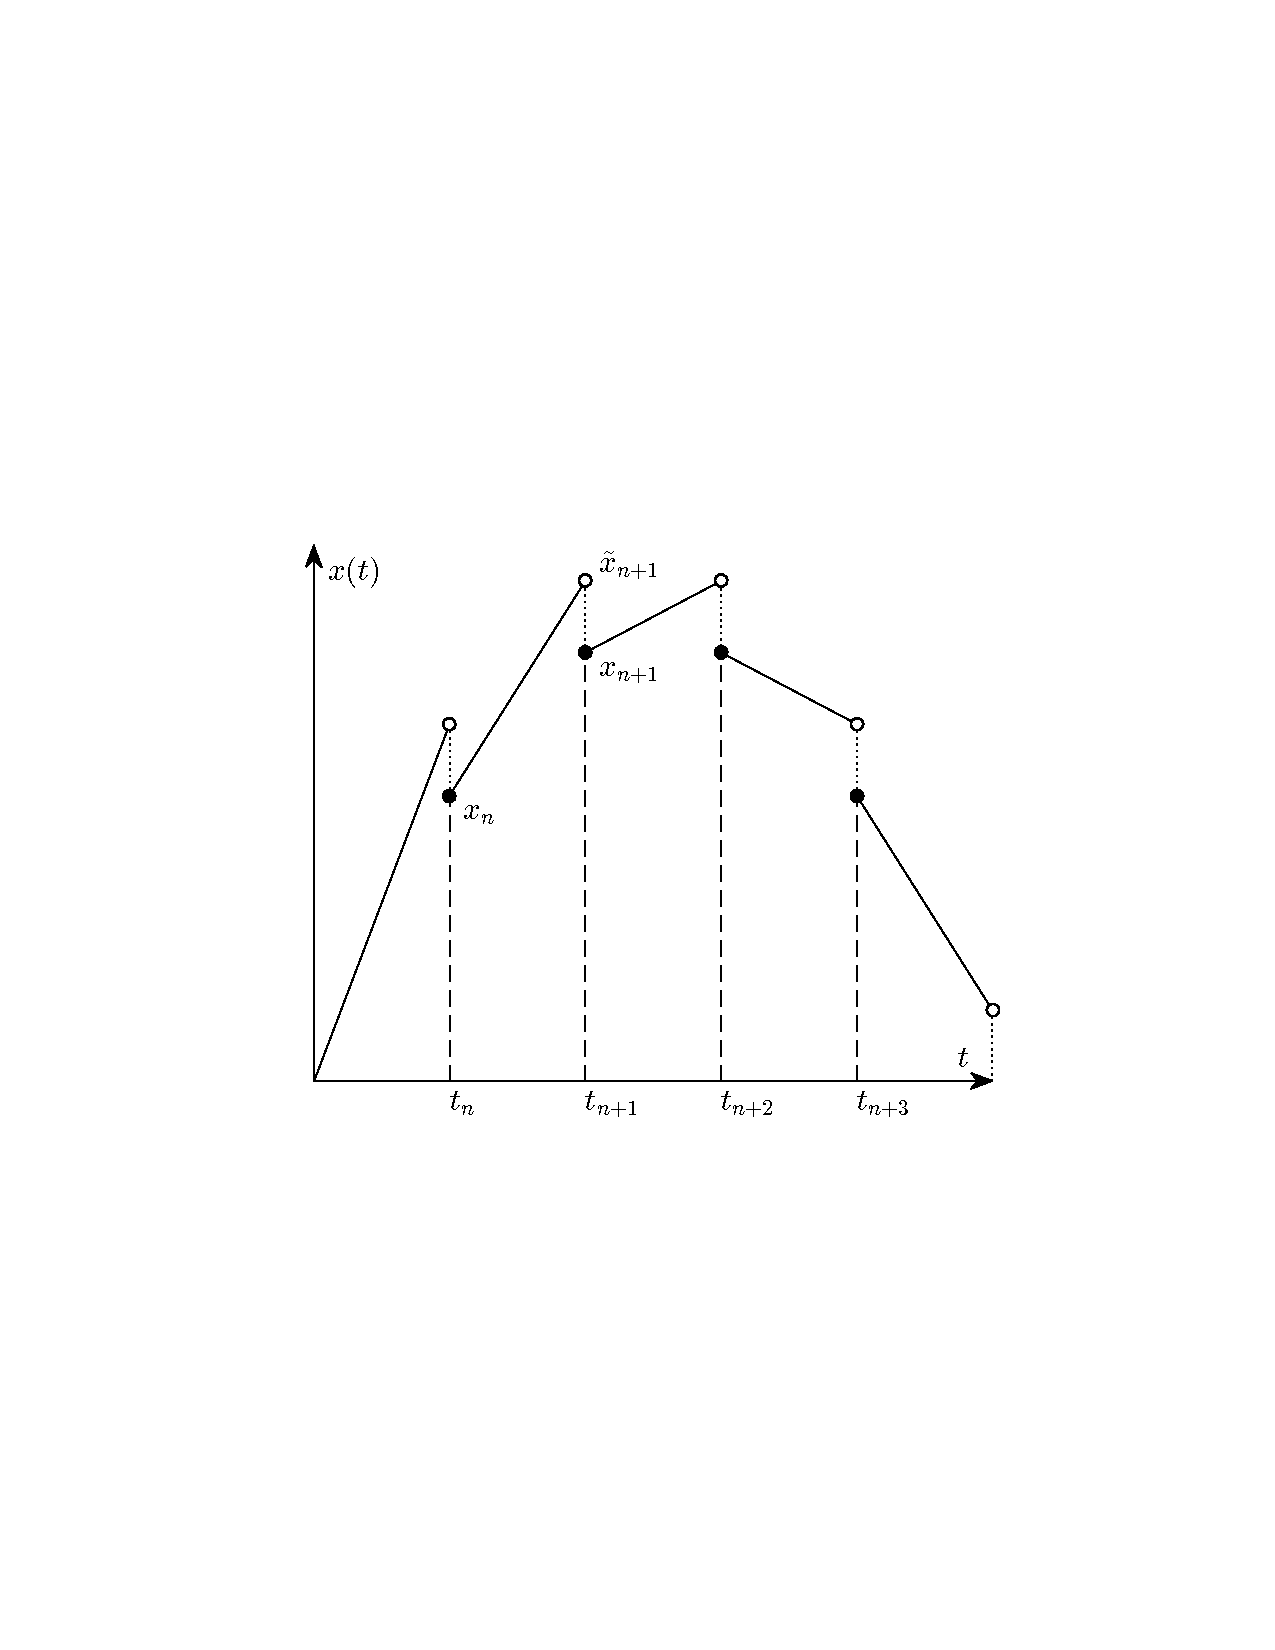
\includegraphics[trim=1cm 5cm 0cm 8cm, clip=true, 
	    width=\linewidth]{img/multShootPlot}
	  \end{center}
	\end{figure}
\end{frame}


